\documentclass[convert]{standalone}

\usepackage{tikz}
\begin{document}
% Created by tikzDevice version 0.12 on 2019-07-02 16:39:15
% !TEX encoding = UTF-8 Unicode
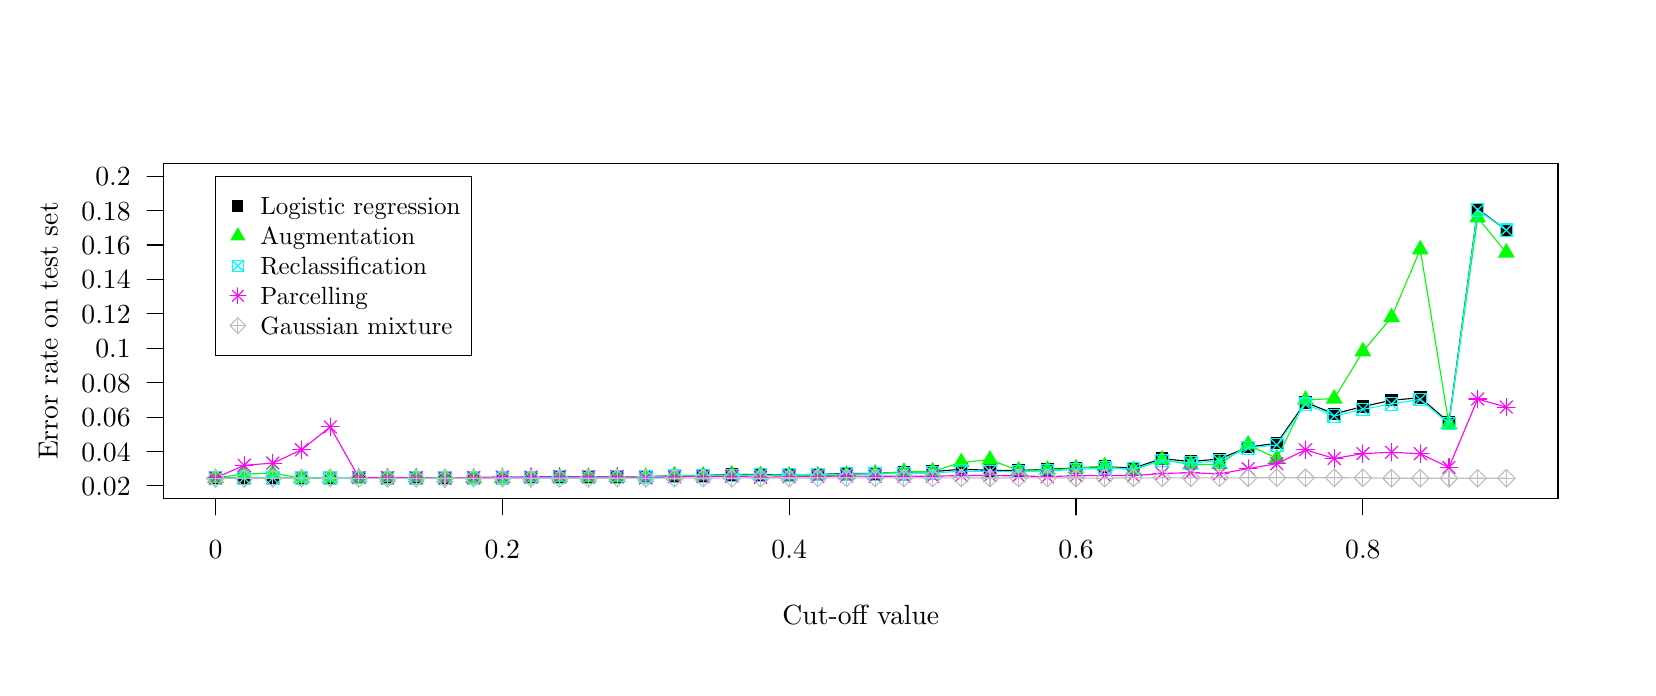
\begin{tikzpicture}[x=1pt,y=1pt]
\definecolor{fillColor}{RGB}{255,255,255}
\path[use as bounding box,fill=fillColor,fill opacity=0.00] (0,0) rectangle (578.16,231.26);
\begin{scope}
\path[clip] ( 49.20, 61.20) rectangle (552.96,182.06);
\definecolor{drawColor}{RGB}{0,0,0}

\path[draw=drawColor,line width= 0.4pt,line join=round,line cap=round] ( 67.86, 68.55) --
	( 78.22, 68.54) --
	( 88.59, 68.40) --
	( 98.95, 68.49) --
	(109.32, 68.56) --
	(119.68, 68.49) --
	(130.05, 68.56) --
	(140.42, 68.56) --
	(150.78, 68.56) --
	(161.15, 68.60) --
	(171.51, 68.69) --
	(181.88, 68.62) --
	(192.24, 68.69) --
	(202.61, 68.77) --
	(212.97, 68.90) --
	(223.34, 69.03) --
	(233.70, 69.35) --
	(244.07, 69.46) --
	(254.44, 69.79) --
	(264.80, 69.79) --
	(275.17, 69.69) --
	(285.53, 69.85) --
	(295.90, 70.17) --
	(306.26, 70.16) --
	(316.63, 70.68) --
	(326.99, 70.82) --
	(337.36, 71.71) --
	(347.72, 71.32) --
	(358.09, 71.28) --
	(368.46, 71.66) --
	(378.82, 72.19) --
	(389.19, 72.63) --
	(399.55, 72.11) --
	(409.92, 75.53) --
	(420.28, 74.46) --
	(430.65, 75.43) --
	(441.01, 79.67) --
	(451.38, 81.13) --
	(461.74, 95.88) --
	(472.11, 91.70) --
	(482.48, 94.35) --
	(492.84, 96.62) --
	(503.21, 97.55) --
	(513.57, 88.67) --
	(523.94,165.74) --
	(534.30,158.10);
\definecolor{fillColor}{RGB}{0,0,0}

\path[fill=fillColor] ( 65.61, 66.30) --
	( 70.11, 66.30) --
	( 70.11, 70.80) --
	( 65.61, 70.80) --
	cycle;

\path[fill=fillColor] ( 75.97, 66.29) --
	( 80.47, 66.29) --
	( 80.47, 70.79) --
	( 75.97, 70.79) --
	cycle;

\path[fill=fillColor] ( 86.34, 66.15) --
	( 90.84, 66.15) --
	( 90.84, 70.65) --
	( 86.34, 70.65) --
	cycle;

\path[fill=fillColor] ( 96.70, 66.24) --
	(101.20, 66.24) --
	(101.20, 70.74) --
	( 96.70, 70.74) --
	cycle;

\path[fill=fillColor] (107.07, 66.31) --
	(111.57, 66.31) --
	(111.57, 70.81) --
	(107.07, 70.81) --
	cycle;

\path[fill=fillColor] (117.43, 66.24) --
	(121.93, 66.24) --
	(121.93, 70.74) --
	(117.43, 70.74) --
	cycle;

\path[fill=fillColor] (127.80, 66.31) --
	(132.30, 66.31) --
	(132.30, 70.81) --
	(127.80, 70.81) --
	cycle;

\path[fill=fillColor] (138.17, 66.31) --
	(142.67, 66.31) --
	(142.67, 70.81) --
	(138.17, 70.81) --
	cycle;

\path[fill=fillColor] (148.53, 66.31) --
	(153.03, 66.31) --
	(153.03, 70.81) --
	(148.53, 70.81) --
	cycle;

\path[fill=fillColor] (158.90, 66.35) --
	(163.40, 66.35) --
	(163.40, 70.85) --
	(158.90, 70.85) --
	cycle;

\path[fill=fillColor] (169.26, 66.44) --
	(173.76, 66.44) --
	(173.76, 70.94) --
	(169.26, 70.94) --
	cycle;

\path[fill=fillColor] (179.63, 66.37) --
	(184.13, 66.37) --
	(184.13, 70.87) --
	(179.63, 70.87) --
	cycle;

\path[fill=fillColor] (189.99, 66.44) --
	(194.49, 66.44) --
	(194.49, 70.94) --
	(189.99, 70.94) --
	cycle;

\path[fill=fillColor] (200.36, 66.52) --
	(204.86, 66.52) --
	(204.86, 71.02) --
	(200.36, 71.02) --
	cycle;

\path[fill=fillColor] (210.72, 66.65) --
	(215.22, 66.65) --
	(215.22, 71.15) --
	(210.72, 71.15) --
	cycle;

\path[fill=fillColor] (221.09, 66.78) --
	(225.59, 66.78) --
	(225.59, 71.28) --
	(221.09, 71.28) --
	cycle;

\path[fill=fillColor] (231.45, 67.10) --
	(235.95, 67.10) --
	(235.95, 71.60) --
	(231.45, 71.60) --
	cycle;

\path[fill=fillColor] (241.82, 67.21) --
	(246.32, 67.21) --
	(246.32, 71.71) --
	(241.82, 71.71) --
	cycle;

\path[fill=fillColor] (252.19, 67.54) --
	(256.69, 67.54) --
	(256.69, 72.04) --
	(252.19, 72.04) --
	cycle;

\path[fill=fillColor] (262.55, 67.54) --
	(267.05, 67.54) --
	(267.05, 72.04) --
	(262.55, 72.04) --
	cycle;

\path[fill=fillColor] (272.92, 67.44) --
	(277.42, 67.44) --
	(277.42, 71.94) --
	(272.92, 71.94) --
	cycle;

\path[fill=fillColor] (283.28, 67.60) --
	(287.78, 67.60) --
	(287.78, 72.10) --
	(283.28, 72.10) --
	cycle;

\path[fill=fillColor] (293.65, 67.92) --
	(298.15, 67.92) --
	(298.15, 72.42) --
	(293.65, 72.42) --
	cycle;

\path[fill=fillColor] (304.01, 67.91) --
	(308.51, 67.91) --
	(308.51, 72.41) --
	(304.01, 72.41) --
	cycle;

\path[fill=fillColor] (314.38, 68.43) --
	(318.88, 68.43) --
	(318.88, 72.93) --
	(314.38, 72.93) --
	cycle;

\path[fill=fillColor] (324.74, 68.57) --
	(329.24, 68.57) --
	(329.24, 73.07) --
	(324.74, 73.07) --
	cycle;

\path[fill=fillColor] (335.11, 69.46) --
	(339.61, 69.46) --
	(339.61, 73.96) --
	(335.11, 73.96) --
	cycle;

\path[fill=fillColor] (345.47, 69.07) --
	(349.97, 69.07) --
	(349.97, 73.57) --
	(345.47, 73.57) --
	cycle;

\path[fill=fillColor] (355.84, 69.03) --
	(360.34, 69.03) --
	(360.34, 73.53) --
	(355.84, 73.53) --
	cycle;

\path[fill=fillColor] (366.21, 69.41) --
	(370.71, 69.41) --
	(370.71, 73.91) --
	(366.21, 73.91) --
	cycle;

\path[fill=fillColor] (376.57, 69.94) --
	(381.07, 69.94) --
	(381.07, 74.44) --
	(376.57, 74.44) --
	cycle;

\path[fill=fillColor] (386.94, 70.38) --
	(391.44, 70.38) --
	(391.44, 74.88) --
	(386.94, 74.88) --
	cycle;

\path[fill=fillColor] (397.30, 69.86) --
	(401.80, 69.86) --
	(401.80, 74.36) --
	(397.30, 74.36) --
	cycle;

\path[fill=fillColor] (407.67, 73.28) --
	(412.17, 73.28) --
	(412.17, 77.78) --
	(407.67, 77.78) --
	cycle;

\path[fill=fillColor] (418.03, 72.21) --
	(422.53, 72.21) --
	(422.53, 76.71) --
	(418.03, 76.71) --
	cycle;

\path[fill=fillColor] (428.40, 73.18) --
	(432.90, 73.18) --
	(432.90, 77.68) --
	(428.40, 77.68) --
	cycle;

\path[fill=fillColor] (438.76, 77.42) --
	(443.26, 77.42) --
	(443.26, 81.92) --
	(438.76, 81.92) --
	cycle;

\path[fill=fillColor] (449.13, 78.88) --
	(453.63, 78.88) --
	(453.63, 83.38) --
	(449.13, 83.38) --
	cycle;

\path[fill=fillColor] (459.49, 93.63) --
	(463.99, 93.63) --
	(463.99, 98.13) --
	(459.49, 98.13) --
	cycle;

\path[fill=fillColor] (469.86, 89.45) --
	(474.36, 89.45) --
	(474.36, 93.95) --
	(469.86, 93.95) --
	cycle;

\path[fill=fillColor] (480.23, 92.10) --
	(484.73, 92.10) --
	(484.73, 96.60) --
	(480.23, 96.60) --
	cycle;

\path[fill=fillColor] (490.59, 94.37) --
	(495.09, 94.37) --
	(495.09, 98.87) --
	(490.59, 98.87) --
	cycle;

\path[fill=fillColor] (500.96, 95.30) --
	(505.46, 95.30) --
	(505.46, 99.80) --
	(500.96, 99.80) --
	cycle;

\path[fill=fillColor] (511.32, 86.42) --
	(515.82, 86.42) --
	(515.82, 90.92) --
	(511.32, 90.92) --
	cycle;

\path[fill=fillColor] (521.69,163.49) --
	(526.19,163.49) --
	(526.19,167.99) --
	(521.69,167.99) --
	cycle;

\path[fill=fillColor] (532.05,155.85) --
	(536.55,155.85) --
	(536.55,160.35) --
	(532.05,160.35) --
	cycle;
\end{scope}
\begin{scope}
\path[clip] (  0.00,  0.00) rectangle (578.16,231.26);
\definecolor{drawColor}{RGB}{0,0,0}

\path[draw=drawColor,line width= 0.4pt,line join=round,line cap=round] ( 49.20, 61.20) --
	(552.96, 61.20) --
	(552.96,182.06) --
	( 49.20,182.06) --
	( 49.20, 61.20);
\end{scope}
\begin{scope}
\path[clip] (  0.00,  0.00) rectangle (578.16,231.26);
\definecolor{drawColor}{RGB}{0,0,0}

\node[text=drawColor,anchor=base,inner sep=0pt, outer sep=0pt, scale=  1.00] at (301.08, 15.60) {Cut-off value};

\node[text=drawColor,rotate= 90.00,anchor=base,inner sep=0pt, outer sep=0pt, scale=  1.00] at ( 10.80,121.63) {Error rate on test set};
\end{scope}
\begin{scope}
\path[clip] ( 49.20, 61.20) rectangle (552.96,182.06);
\definecolor{drawColor}{RGB}{0,255,0}

\path[draw=drawColor,line width= 0.4pt,line join=round,line cap=round] ( 67.86, 68.55) --
	( 78.22, 69.97) --
	( 88.59, 70.22) --
	( 98.95, 68.50) --
	(109.32, 68.59) --
	(119.68, 68.62) --
	(130.05, 68.75) --
	(140.42, 68.80) --
	(150.78, 68.59) --
	(161.15, 68.53) --
	(171.51, 68.49) --
	(181.88, 68.72) --
	(192.24, 68.83) --
	(202.61, 68.79) --
	(212.97, 68.82) --
	(223.34, 68.95) --
	(233.70, 69.43) --
	(244.07, 69.41) --
	(254.44, 69.77) --
	(264.80, 69.54) --
	(275.17, 69.33) --
	(285.53, 69.39) --
	(295.90, 69.65) --
	(306.26, 70.13) --
	(316.63, 70.74) --
	(326.99, 70.85) --
	(337.36, 74.20) --
	(347.72, 75.15) --
	(358.09, 71.21) --
	(368.46, 71.50) --
	(378.82, 72.01) --
	(389.19, 72.80) --
	(399.55, 71.35) --
	(409.92, 75.16) --
	(420.28, 73.40) --
	(430.65, 73.47) --
	(441.01, 80.59) --
	(451.38, 75.56) --
	(461.74, 96.78) --
	(472.11, 97.20) --
	(482.48,114.26) --
	(492.84,126.62) --
	(503.21,151.11) --
	(513.57, 88.00) --
	(523.94,162.63) --
	(534.30,149.95);
\definecolor{fillColor}{RGB}{0,255,0}

\path[fill=fillColor] ( 67.86, 72.05) --
	( 70.89, 66.80) --
	( 64.83, 66.80) --
	cycle;

\path[fill=fillColor] ( 78.22, 73.47) --
	( 81.25, 68.22) --
	( 75.19, 68.22) --
	cycle;

\path[fill=fillColor] ( 88.59, 73.72) --
	( 91.62, 68.47) --
	( 85.56, 68.47) --
	cycle;

\path[fill=fillColor] ( 98.95, 72.00) --
	(101.98, 66.75) --
	( 95.92, 66.75) --
	cycle;

\path[fill=fillColor] (109.32, 72.09) --
	(112.35, 66.84) --
	(106.29, 66.84) --
	cycle;

\path[fill=fillColor] (119.68, 72.12) --
	(122.72, 66.87) --
	(116.65, 66.87) --
	cycle;

\path[fill=fillColor] (130.05, 72.25) --
	(133.08, 67.00) --
	(127.02, 67.00) --
	cycle;

\path[fill=fillColor] (140.42, 72.30) --
	(143.45, 67.05) --
	(137.39, 67.05) --
	cycle;

\path[fill=fillColor] (150.78, 72.09) --
	(153.81, 66.84) --
	(147.75, 66.84) --
	cycle;

\path[fill=fillColor] (161.15, 72.03) --
	(164.18, 66.78) --
	(158.12, 66.78) --
	cycle;

\path[fill=fillColor] (171.51, 71.99) --
	(174.54, 66.74) --
	(168.48, 66.74) --
	cycle;

\path[fill=fillColor] (181.88, 72.22) --
	(184.91, 66.97) --
	(178.85, 66.97) --
	cycle;

\path[fill=fillColor] (192.24, 72.33) --
	(195.27, 67.08) --
	(189.21, 67.08) --
	cycle;

\path[fill=fillColor] (202.61, 72.28) --
	(205.64, 67.04) --
	(199.58, 67.04) --
	cycle;

\path[fill=fillColor] (212.97, 72.32) --
	(216.00, 67.07) --
	(209.94, 67.07) --
	cycle;

\path[fill=fillColor] (223.34, 72.45) --
	(226.37, 67.20) --
	(220.31, 67.20) --
	cycle;

\path[fill=fillColor] (233.70, 72.92) --
	(236.73, 67.68) --
	(230.67, 67.68) --
	cycle;

\path[fill=fillColor] (244.07, 72.91) --
	(247.10, 67.66) --
	(241.04, 67.66) --
	cycle;

\path[fill=fillColor] (254.44, 73.27) --
	(257.47, 68.02) --
	(251.41, 68.02) --
	cycle;

\path[fill=fillColor] (264.80, 73.04) --
	(267.83, 67.79) --
	(261.77, 67.79) --
	cycle;

\path[fill=fillColor] (275.17, 72.83) --
	(278.20, 67.58) --
	(272.14, 67.58) --
	cycle;

\path[fill=fillColor] (285.53, 72.89) --
	(288.56, 67.64) --
	(282.50, 67.64) --
	cycle;

\path[fill=fillColor] (295.90, 73.15) --
	(298.93, 67.90) --
	(292.87, 67.90) --
	cycle;

\path[fill=fillColor] (306.26, 73.63) --
	(309.29, 68.38) --
	(303.23, 68.38) --
	cycle;

\path[fill=fillColor] (316.63, 74.24) --
	(319.66, 68.99) --
	(313.60, 68.99) --
	cycle;

\path[fill=fillColor] (326.99, 74.35) --
	(330.02, 69.10) --
	(323.96, 69.10) --
	cycle;

\path[fill=fillColor] (337.36, 77.70) --
	(340.39, 72.45) --
	(334.33, 72.45) --
	cycle;

\path[fill=fillColor] (347.72, 78.64) --
	(350.75, 73.40) --
	(344.69, 73.40) --
	cycle;

\path[fill=fillColor] (358.09, 74.71) --
	(361.12, 69.46) --
	(355.06, 69.46) --
	cycle;

\path[fill=fillColor] (368.46, 75.00) --
	(371.49, 69.75) --
	(365.43, 69.75) --
	cycle;

\path[fill=fillColor] (378.82, 75.50) --
	(381.85, 70.26) --
	(375.79, 70.26) --
	cycle;

\path[fill=fillColor] (389.19, 76.29) --
	(392.22, 71.05) --
	(386.16, 71.05) --
	cycle;

\path[fill=fillColor] (399.55, 74.85) --
	(402.58, 69.60) --
	(396.52, 69.60) --
	cycle;

\path[fill=fillColor] (409.92, 78.66) --
	(412.95, 73.41) --
	(406.89, 73.41) --
	cycle;

\path[fill=fillColor] (420.28, 76.90) --
	(423.31, 71.66) --
	(417.25, 71.66) --
	cycle;

\path[fill=fillColor] (430.65, 76.97) --
	(433.68, 71.72) --
	(427.62, 71.72) --
	cycle;

\path[fill=fillColor] (441.01, 84.09) --
	(444.04, 78.84) --
	(437.98, 78.84) --
	cycle;

\path[fill=fillColor] (451.38, 79.05) --
	(454.41, 73.81) --
	(448.35, 73.81) --
	cycle;

\path[fill=fillColor] (461.74,100.27) --
	(464.77, 95.03) --
	(458.71, 95.03) --
	cycle;

\path[fill=fillColor] (472.11,100.70) --
	(475.14, 95.45) --
	(469.08, 95.45) --
	cycle;

\path[fill=fillColor] (482.48,117.76) --
	(485.51,112.52) --
	(479.44,112.52) --
	cycle;

\path[fill=fillColor] (492.84,130.12) --
	(495.87,124.87) --
	(489.81,124.87) --
	cycle;

\path[fill=fillColor] (503.21,154.61) --
	(506.24,149.36) --
	(500.18,149.36) --
	cycle;

\path[fill=fillColor] (513.57, 91.50) --
	(516.60, 86.25) --
	(510.54, 86.25) --
	cycle;

\path[fill=fillColor] (523.94,166.13) --
	(526.97,160.88) --
	(520.91,160.88) --
	cycle;

\path[fill=fillColor] (534.30,153.45) --
	(537.33,148.20) --
	(531.27,148.20) --
	cycle;
\end{scope}
\begin{scope}
\path[clip] (  0.00,  0.00) rectangle (578.16,231.26);
\definecolor{drawColor}{RGB}{0,0,0}

\path[draw=drawColor,line width= 0.4pt,line join=round,line cap=round] ( 49.20, 61.20) --
	(552.96, 61.20) --
	(552.96,182.06) --
	( 49.20,182.06) --
	( 49.20, 61.20);
\end{scope}
\begin{scope}
\path[clip] (  0.00,  0.00) rectangle (578.16,231.26);
\definecolor{drawColor}{RGB}{0,0,0}

%\node[text=drawColor,anchor=base,inner sep=0pt, outer sep=0pt, scale=  1.00] at (301.08, 15.60) {Cut-off value};

%\node[text=drawColor,rotate= 90.00,anchor=base,inner sep=0pt, outer sep=0pt, scale=  1.00] at ( 10.80,121.63) {Error rate on test set};
\end{scope}
\begin{scope}
\path[clip] ( 49.20, 61.20) rectangle (552.96,182.06);
\definecolor{drawColor}{RGB}{0,255,255}

\path[draw=drawColor,line width= 0.4pt,line join=round,line cap=round] ( 67.86, 68.55) --
	( 78.22, 68.51) --
	( 88.59, 68.52) --
	( 98.95, 68.56) --
	(109.32, 68.59) --
	(119.68, 68.64) --
	(130.05, 68.61) --
	(140.42, 68.60) --
	(150.78, 68.59) --
	(161.15, 68.61) --
	(171.51, 68.61) --
	(181.88, 68.69) --
	(192.24, 68.85) --
	(202.61, 68.85) --
	(212.97, 68.92) --
	(223.34, 68.98) --
	(233.70, 69.16) --
	(244.07, 69.31) --
	(254.44, 69.43) --
	(264.80, 69.57) --
	(275.17, 69.64) --
	(285.53, 69.82) --
	(295.90, 70.01) --
	(306.26, 69.98) --
	(316.63, 70.06) --
	(326.99, 70.30) --
	(337.36, 71.00) --
	(347.72, 70.89) --
	(358.09, 70.81) --
	(368.46, 71.05) --
	(378.82, 71.61) --
	(389.19, 72.17) --
	(399.55, 71.79) --
	(409.92, 74.87) --
	(420.28, 73.96) --
	(430.65, 74.69) --
	(441.01, 79.39) --
	(451.38, 80.44) --
	(461.74, 95.21) --
	(472.11, 90.92) --
	(482.48, 93.36) --
	(492.84, 95.30) --
	(503.21, 96.93) --
	(513.57, 88.18) --
	(523.94,165.41) --
	(534.30,158.07);

\path[draw=drawColor,line width= 0.4pt,line join=round,line cap=round] ( 65.61, 66.30) rectangle ( 70.11, 70.80);

\path[draw=drawColor,line width= 0.4pt,line join=round,line cap=round] ( 65.61, 66.30) -- ( 70.11, 70.80);

\path[draw=drawColor,line width= 0.4pt,line join=round,line cap=round] ( 65.61, 70.80) -- ( 70.11, 66.30);

\path[draw=drawColor,line width= 0.4pt,line join=round,line cap=round] ( 75.97, 66.26) rectangle ( 80.47, 70.76);

\path[draw=drawColor,line width= 0.4pt,line join=round,line cap=round] ( 75.97, 66.26) -- ( 80.47, 70.76);

\path[draw=drawColor,line width= 0.4pt,line join=round,line cap=round] ( 75.97, 70.76) -- ( 80.47, 66.26);

\path[draw=drawColor,line width= 0.4pt,line join=round,line cap=round] ( 86.34, 66.27) rectangle ( 90.84, 70.77);

\path[draw=drawColor,line width= 0.4pt,line join=round,line cap=round] ( 86.34, 66.27) -- ( 90.84, 70.77);

\path[draw=drawColor,line width= 0.4pt,line join=round,line cap=round] ( 86.34, 70.77) -- ( 90.84, 66.27);

\path[draw=drawColor,line width= 0.4pt,line join=round,line cap=round] ( 96.70, 66.31) rectangle (101.20, 70.81);

\path[draw=drawColor,line width= 0.4pt,line join=round,line cap=round] ( 96.70, 66.31) -- (101.20, 70.81);

\path[draw=drawColor,line width= 0.4pt,line join=round,line cap=round] ( 96.70, 70.81) -- (101.20, 66.31);

\path[draw=drawColor,line width= 0.4pt,line join=round,line cap=round] (107.07, 66.34) rectangle (111.57, 70.84);

\path[draw=drawColor,line width= 0.4pt,line join=round,line cap=round] (107.07, 66.34) -- (111.57, 70.84);

\path[draw=drawColor,line width= 0.4pt,line join=round,line cap=round] (107.07, 70.84) -- (111.57, 66.34);

\path[draw=drawColor,line width= 0.4pt,line join=round,line cap=round] (117.43, 66.39) rectangle (121.93, 70.89);

\path[draw=drawColor,line width= 0.4pt,line join=round,line cap=round] (117.43, 66.39) -- (121.93, 70.89);

\path[draw=drawColor,line width= 0.4pt,line join=round,line cap=round] (117.43, 70.89) -- (121.93, 66.39);

\path[draw=drawColor,line width= 0.4pt,line join=round,line cap=round] (127.80, 66.36) rectangle (132.30, 70.86);

\path[draw=drawColor,line width= 0.4pt,line join=round,line cap=round] (127.80, 66.36) -- (132.30, 70.86);

\path[draw=drawColor,line width= 0.4pt,line join=round,line cap=round] (127.80, 70.86) -- (132.30, 66.36);

\path[draw=drawColor,line width= 0.4pt,line join=round,line cap=round] (138.17, 66.35) rectangle (142.67, 70.85);

\path[draw=drawColor,line width= 0.4pt,line join=round,line cap=round] (138.17, 66.35) -- (142.67, 70.85);

\path[draw=drawColor,line width= 0.4pt,line join=round,line cap=round] (138.17, 70.85) -- (142.67, 66.35);

\path[draw=drawColor,line width= 0.4pt,line join=round,line cap=round] (148.53, 66.34) rectangle (153.03, 70.84);

\path[draw=drawColor,line width= 0.4pt,line join=round,line cap=round] (148.53, 66.34) -- (153.03, 70.84);

\path[draw=drawColor,line width= 0.4pt,line join=round,line cap=round] (148.53, 70.84) -- (153.03, 66.34);

\path[draw=drawColor,line width= 0.4pt,line join=round,line cap=round] (158.90, 66.36) rectangle (163.40, 70.86);

\path[draw=drawColor,line width= 0.4pt,line join=round,line cap=round] (158.90, 66.36) -- (163.40, 70.86);

\path[draw=drawColor,line width= 0.4pt,line join=round,line cap=round] (158.90, 70.86) -- (163.40, 66.36);

\path[draw=drawColor,line width= 0.4pt,line join=round,line cap=round] (169.26, 66.36) rectangle (173.76, 70.86);

\path[draw=drawColor,line width= 0.4pt,line join=round,line cap=round] (169.26, 66.36) -- (173.76, 70.86);

\path[draw=drawColor,line width= 0.4pt,line join=round,line cap=round] (169.26, 70.86) -- (173.76, 66.36);

\path[draw=drawColor,line width= 0.4pt,line join=round,line cap=round] (179.63, 66.44) rectangle (184.13, 70.94);

\path[draw=drawColor,line width= 0.4pt,line join=round,line cap=round] (179.63, 66.44) -- (184.13, 70.94);

\path[draw=drawColor,line width= 0.4pt,line join=round,line cap=round] (179.63, 70.94) -- (184.13, 66.44);

\path[draw=drawColor,line width= 0.4pt,line join=round,line cap=round] (189.99, 66.60) rectangle (194.49, 71.10);

\path[draw=drawColor,line width= 0.4pt,line join=round,line cap=round] (189.99, 66.60) -- (194.49, 71.10);

\path[draw=drawColor,line width= 0.4pt,line join=round,line cap=round] (189.99, 71.10) -- (194.49, 66.60);

\path[draw=drawColor,line width= 0.4pt,line join=round,line cap=round] (200.36, 66.60) rectangle (204.86, 71.10);

\path[draw=drawColor,line width= 0.4pt,line join=round,line cap=round] (200.36, 66.60) -- (204.86, 71.10);

\path[draw=drawColor,line width= 0.4pt,line join=round,line cap=round] (200.36, 71.10) -- (204.86, 66.60);

\path[draw=drawColor,line width= 0.4pt,line join=round,line cap=round] (210.72, 66.67) rectangle (215.22, 71.17);

\path[draw=drawColor,line width= 0.4pt,line join=round,line cap=round] (210.72, 66.67) -- (215.22, 71.17);

\path[draw=drawColor,line width= 0.4pt,line join=round,line cap=round] (210.72, 71.17) -- (215.22, 66.67);

\path[draw=drawColor,line width= 0.4pt,line join=round,line cap=round] (221.09, 66.73) rectangle (225.59, 71.23);

\path[draw=drawColor,line width= 0.4pt,line join=round,line cap=round] (221.09, 66.73) -- (225.59, 71.23);

\path[draw=drawColor,line width= 0.4pt,line join=round,line cap=round] (221.09, 71.23) -- (225.59, 66.73);

\path[draw=drawColor,line width= 0.4pt,line join=round,line cap=round] (231.45, 66.91) rectangle (235.95, 71.41);

\path[draw=drawColor,line width= 0.4pt,line join=round,line cap=round] (231.45, 66.91) -- (235.95, 71.41);

\path[draw=drawColor,line width= 0.4pt,line join=round,line cap=round] (231.45, 71.41) -- (235.95, 66.91);

\path[draw=drawColor,line width= 0.4pt,line join=round,line cap=round] (241.82, 67.06) rectangle (246.32, 71.56);

\path[draw=drawColor,line width= 0.4pt,line join=round,line cap=round] (241.82, 67.06) -- (246.32, 71.56);

\path[draw=drawColor,line width= 0.4pt,line join=round,line cap=round] (241.82, 71.56) -- (246.32, 67.06);

\path[draw=drawColor,line width= 0.4pt,line join=round,line cap=round] (252.19, 67.18) rectangle (256.69, 71.68);

\path[draw=drawColor,line width= 0.4pt,line join=round,line cap=round] (252.19, 67.18) -- (256.69, 71.68);

\path[draw=drawColor,line width= 0.4pt,line join=round,line cap=round] (252.19, 71.68) -- (256.69, 67.18);

\path[draw=drawColor,line width= 0.4pt,line join=round,line cap=round] (262.55, 67.32) rectangle (267.05, 71.82);

\path[draw=drawColor,line width= 0.4pt,line join=round,line cap=round] (262.55, 67.32) -- (267.05, 71.82);

\path[draw=drawColor,line width= 0.4pt,line join=round,line cap=round] (262.55, 71.82) -- (267.05, 67.32);

\path[draw=drawColor,line width= 0.4pt,line join=round,line cap=round] (272.92, 67.39) rectangle (277.42, 71.89);

\path[draw=drawColor,line width= 0.4pt,line join=round,line cap=round] (272.92, 67.39) -- (277.42, 71.89);

\path[draw=drawColor,line width= 0.4pt,line join=round,line cap=round] (272.92, 71.89) -- (277.42, 67.39);

\path[draw=drawColor,line width= 0.4pt,line join=round,line cap=round] (283.28, 67.57) rectangle (287.78, 72.07);

\path[draw=drawColor,line width= 0.4pt,line join=round,line cap=round] (283.28, 67.57) -- (287.78, 72.07);

\path[draw=drawColor,line width= 0.4pt,line join=round,line cap=round] (283.28, 72.07) -- (287.78, 67.57);

\path[draw=drawColor,line width= 0.4pt,line join=round,line cap=round] (293.65, 67.76) rectangle (298.15, 72.26);

\path[draw=drawColor,line width= 0.4pt,line join=round,line cap=round] (293.65, 67.76) -- (298.15, 72.26);

\path[draw=drawColor,line width= 0.4pt,line join=round,line cap=round] (293.65, 72.26) -- (298.15, 67.76);

\path[draw=drawColor,line width= 0.4pt,line join=round,line cap=round] (304.01, 67.73) rectangle (308.51, 72.23);

\path[draw=drawColor,line width= 0.4pt,line join=round,line cap=round] (304.01, 67.73) -- (308.51, 72.23);

\path[draw=drawColor,line width= 0.4pt,line join=round,line cap=round] (304.01, 72.23) -- (308.51, 67.73);

\path[draw=drawColor,line width= 0.4pt,line join=round,line cap=round] (314.38, 67.81) rectangle (318.88, 72.31);

\path[draw=drawColor,line width= 0.4pt,line join=round,line cap=round] (314.38, 67.81) -- (318.88, 72.31);

\path[draw=drawColor,line width= 0.4pt,line join=round,line cap=round] (314.38, 72.31) -- (318.88, 67.81);

\path[draw=drawColor,line width= 0.4pt,line join=round,line cap=round] (324.74, 68.05) rectangle (329.24, 72.55);

\path[draw=drawColor,line width= 0.4pt,line join=round,line cap=round] (324.74, 68.05) -- (329.24, 72.55);

\path[draw=drawColor,line width= 0.4pt,line join=round,line cap=round] (324.74, 72.55) -- (329.24, 68.05);

\path[draw=drawColor,line width= 0.4pt,line join=round,line cap=round] (335.11, 68.75) rectangle (339.61, 73.25);

\path[draw=drawColor,line width= 0.4pt,line join=round,line cap=round] (335.11, 68.75) -- (339.61, 73.25);

\path[draw=drawColor,line width= 0.4pt,line join=round,line cap=round] (335.11, 73.25) -- (339.61, 68.75);

\path[draw=drawColor,line width= 0.4pt,line join=round,line cap=round] (345.47, 68.64) rectangle (349.97, 73.14);

\path[draw=drawColor,line width= 0.4pt,line join=round,line cap=round] (345.47, 68.64) -- (349.97, 73.14);

\path[draw=drawColor,line width= 0.4pt,line join=round,line cap=round] (345.47, 73.14) -- (349.97, 68.64);

\path[draw=drawColor,line width= 0.4pt,line join=round,line cap=round] (355.84, 68.56) rectangle (360.34, 73.06);

\path[draw=drawColor,line width= 0.4pt,line join=round,line cap=round] (355.84, 68.56) -- (360.34, 73.06);

\path[draw=drawColor,line width= 0.4pt,line join=round,line cap=round] (355.84, 73.06) -- (360.34, 68.56);

\path[draw=drawColor,line width= 0.4pt,line join=round,line cap=round] (366.21, 68.80) rectangle (370.71, 73.30);

\path[draw=drawColor,line width= 0.4pt,line join=round,line cap=round] (366.21, 68.80) -- (370.71, 73.30);

\path[draw=drawColor,line width= 0.4pt,line join=round,line cap=round] (366.21, 73.30) -- (370.71, 68.80);

\path[draw=drawColor,line width= 0.4pt,line join=round,line cap=round] (376.57, 69.36) rectangle (381.07, 73.86);

\path[draw=drawColor,line width= 0.4pt,line join=round,line cap=round] (376.57, 69.36) -- (381.07, 73.86);

\path[draw=drawColor,line width= 0.4pt,line join=round,line cap=round] (376.57, 73.86) -- (381.07, 69.36);

\path[draw=drawColor,line width= 0.4pt,line join=round,line cap=round] (386.94, 69.92) rectangle (391.44, 74.42);

\path[draw=drawColor,line width= 0.4pt,line join=round,line cap=round] (386.94, 69.92) -- (391.44, 74.42);

\path[draw=drawColor,line width= 0.4pt,line join=round,line cap=round] (386.94, 74.42) -- (391.44, 69.92);

\path[draw=drawColor,line width= 0.4pt,line join=round,line cap=round] (397.30, 69.54) rectangle (401.80, 74.04);

\path[draw=drawColor,line width= 0.4pt,line join=round,line cap=round] (397.30, 69.54) -- (401.80, 74.04);

\path[draw=drawColor,line width= 0.4pt,line join=round,line cap=round] (397.30, 74.04) -- (401.80, 69.54);

\path[draw=drawColor,line width= 0.4pt,line join=round,line cap=round] (407.67, 72.62) rectangle (412.17, 77.12);

\path[draw=drawColor,line width= 0.4pt,line join=round,line cap=round] (407.67, 72.62) -- (412.17, 77.12);

\path[draw=drawColor,line width= 0.4pt,line join=round,line cap=round] (407.67, 77.12) -- (412.17, 72.62);

\path[draw=drawColor,line width= 0.4pt,line join=round,line cap=round] (418.03, 71.71) rectangle (422.53, 76.21);

\path[draw=drawColor,line width= 0.4pt,line join=round,line cap=round] (418.03, 71.71) -- (422.53, 76.21);

\path[draw=drawColor,line width= 0.4pt,line join=round,line cap=round] (418.03, 76.21) -- (422.53, 71.71);

\path[draw=drawColor,line width= 0.4pt,line join=round,line cap=round] (428.40, 72.44) rectangle (432.90, 76.94);

\path[draw=drawColor,line width= 0.4pt,line join=round,line cap=round] (428.40, 72.44) -- (432.90, 76.94);

\path[draw=drawColor,line width= 0.4pt,line join=round,line cap=round] (428.40, 76.94) -- (432.90, 72.44);

\path[draw=drawColor,line width= 0.4pt,line join=round,line cap=round] (438.76, 77.14) rectangle (443.26, 81.64);

\path[draw=drawColor,line width= 0.4pt,line join=round,line cap=round] (438.76, 77.14) -- (443.26, 81.64);

\path[draw=drawColor,line width= 0.4pt,line join=round,line cap=round] (438.76, 81.64) -- (443.26, 77.14);

\path[draw=drawColor,line width= 0.4pt,line join=round,line cap=round] (449.13, 78.19) rectangle (453.63, 82.69);

\path[draw=drawColor,line width= 0.4pt,line join=round,line cap=round] (449.13, 78.19) -- (453.63, 82.69);

\path[draw=drawColor,line width= 0.4pt,line join=round,line cap=round] (449.13, 82.69) -- (453.63, 78.19);

\path[draw=drawColor,line width= 0.4pt,line join=round,line cap=round] (459.49, 92.96) rectangle (463.99, 97.46);

\path[draw=drawColor,line width= 0.4pt,line join=round,line cap=round] (459.49, 92.96) -- (463.99, 97.46);

\path[draw=drawColor,line width= 0.4pt,line join=round,line cap=round] (459.49, 97.46) -- (463.99, 92.96);

\path[draw=drawColor,line width= 0.4pt,line join=round,line cap=round] (469.86, 88.67) rectangle (474.36, 93.17);

\path[draw=drawColor,line width= 0.4pt,line join=round,line cap=round] (469.86, 88.67) -- (474.36, 93.17);

\path[draw=drawColor,line width= 0.4pt,line join=round,line cap=round] (469.86, 93.17) -- (474.36, 88.67);

\path[draw=drawColor,line width= 0.4pt,line join=round,line cap=round] (480.23, 91.11) rectangle (484.73, 95.61);

\path[draw=drawColor,line width= 0.4pt,line join=round,line cap=round] (480.23, 91.11) -- (484.73, 95.61);

\path[draw=drawColor,line width= 0.4pt,line join=round,line cap=round] (480.23, 95.61) -- (484.73, 91.11);

\path[draw=drawColor,line width= 0.4pt,line join=round,line cap=round] (490.59, 93.05) rectangle (495.09, 97.55);

\path[draw=drawColor,line width= 0.4pt,line join=round,line cap=round] (490.59, 93.05) -- (495.09, 97.55);

\path[draw=drawColor,line width= 0.4pt,line join=round,line cap=round] (490.59, 97.55) -- (495.09, 93.05);

\path[draw=drawColor,line width= 0.4pt,line join=round,line cap=round] (500.96, 94.68) rectangle (505.46, 99.18);

\path[draw=drawColor,line width= 0.4pt,line join=round,line cap=round] (500.96, 94.68) -- (505.46, 99.18);

\path[draw=drawColor,line width= 0.4pt,line join=round,line cap=round] (500.96, 99.18) -- (505.46, 94.68);

\path[draw=drawColor,line width= 0.4pt,line join=round,line cap=round] (511.32, 85.93) rectangle (515.82, 90.43);

\path[draw=drawColor,line width= 0.4pt,line join=round,line cap=round] (511.32, 85.93) -- (515.82, 90.43);

\path[draw=drawColor,line width= 0.4pt,line join=round,line cap=round] (511.32, 90.43) -- (515.82, 85.93);

\path[draw=drawColor,line width= 0.4pt,line join=round,line cap=round] (521.69,163.16) rectangle (526.19,167.66);

\path[draw=drawColor,line width= 0.4pt,line join=round,line cap=round] (521.69,163.16) -- (526.19,167.66);

\path[draw=drawColor,line width= 0.4pt,line join=round,line cap=round] (521.69,167.66) -- (526.19,163.16);

\path[draw=drawColor,line width= 0.4pt,line join=round,line cap=round] (532.05,155.82) rectangle (536.55,160.32);

\path[draw=drawColor,line width= 0.4pt,line join=round,line cap=round] (532.05,155.82) -- (536.55,160.32);

\path[draw=drawColor,line width= 0.4pt,line join=round,line cap=round] (532.05,160.32) -- (536.55,155.82);
\end{scope}
\begin{scope}
\path[clip] (  0.00,  0.00) rectangle (578.16,231.26);
\definecolor{drawColor}{RGB}{0,0,0}

\path[draw=drawColor,line width= 0.4pt,line join=round,line cap=round] ( 49.20, 61.20) --
	(552.96, 61.20) --
	(552.96,182.06) --
	( 49.20,182.06) --
	( 49.20, 61.20);
\end{scope}
\begin{scope}
\path[clip] (  0.00,  0.00) rectangle (578.16,231.26);
\definecolor{drawColor}{RGB}{0,0,0}

%\node[text=drawColor,anchor=base,inner sep=0pt, outer sep=0pt, scale=  1.00] at (301.08, 15.60) {Cut-off value};

%\node[text=drawColor,rotate= 90.00,anchor=base,inner sep=0pt, outer sep=0pt, scale=  1.00] at ( 10.80,121.63) {Error rate on test set};
\end{scope}
\begin{scope}
\path[clip] ( 49.20, 61.20) rectangle (552.96,182.06);
\definecolor{drawColor}{RGB}{255,0,255}

\path[draw=drawColor,line width= 0.4pt,line join=round,line cap=round] ( 67.86, 68.55) --
	( 78.22, 73.11) --
	( 88.59, 73.92) --
	( 98.95, 78.73) --
	(109.32, 87.00) --
	(119.68, 68.70) --
	(130.05, 68.69) --
	(140.42, 68.60) --
	(150.78, 68.42) --
	(161.15, 68.74) --
	(171.51, 68.92) --
	(181.88, 68.94) --
	(192.24, 69.12) --
	(202.61, 68.97) --
	(212.97, 69.10) --
	(223.34, 68.56) --
	(233.70, 69.00) --
	(244.07, 69.01) --
	(254.44, 69.18) --
	(264.80, 68.80) --
	(275.17, 68.97) --
	(285.53, 69.12) --
	(295.90, 69.26) --
	(306.26, 69.16) --
	(316.63, 69.20) --
	(326.99, 69.16) --
	(337.36, 69.44) --
	(347.72, 69.41) --
	(358.09, 69.31) --
	(368.46, 69.02) --
	(378.82, 69.34) --
	(389.19, 69.41) --
	(399.55, 69.36) --
	(409.92, 70.17) --
	(420.28, 70.43) --
	(430.65, 70.03) --
	(441.01, 71.91) --
	(451.38, 73.72) --
	(461.74, 78.70) --
	(472.11, 75.59) --
	(482.48, 77.35) --
	(492.84, 77.84) --
	(503.21, 77.30) --
	(513.57, 72.35) --
	(523.94, 97.07) --
	(534.30, 94.15);

\path[draw=drawColor,line width= 0.4pt,line join=round,line cap=round] ( 65.61, 66.30) -- ( 70.11, 70.80);

\path[draw=drawColor,line width= 0.4pt,line join=round,line cap=round] ( 65.61, 70.80) -- ( 70.11, 66.30);

\path[draw=drawColor,line width= 0.4pt,line join=round,line cap=round] ( 64.68, 68.55) -- ( 71.04, 68.55);

\path[draw=drawColor,line width= 0.4pt,line join=round,line cap=round] ( 67.86, 65.37) -- ( 67.86, 71.73);

\path[draw=drawColor,line width= 0.4pt,line join=round,line cap=round] ( 75.97, 70.86) -- ( 80.47, 75.36);

\path[draw=drawColor,line width= 0.4pt,line join=round,line cap=round] ( 75.97, 75.36) -- ( 80.47, 70.86);

\path[draw=drawColor,line width= 0.4pt,line join=round,line cap=round] ( 75.04, 73.11) -- ( 81.41, 73.11);

\path[draw=drawColor,line width= 0.4pt,line join=round,line cap=round] ( 78.22, 69.93) -- ( 78.22, 76.29);

\path[draw=drawColor,line width= 0.4pt,line join=round,line cap=round] ( 86.34, 71.67) -- ( 90.84, 76.17);

\path[draw=drawColor,line width= 0.4pt,line join=round,line cap=round] ( 86.34, 76.17) -- ( 90.84, 71.67);

\path[draw=drawColor,line width= 0.4pt,line join=round,line cap=round] ( 85.41, 73.92) -- ( 91.77, 73.92);

\path[draw=drawColor,line width= 0.4pt,line join=round,line cap=round] ( 88.59, 70.74) -- ( 88.59, 77.10);

\path[draw=drawColor,line width= 0.4pt,line join=round,line cap=round] ( 96.70, 76.48) -- (101.20, 80.98);

\path[draw=drawColor,line width= 0.4pt,line join=round,line cap=round] ( 96.70, 80.98) -- (101.20, 76.48);

\path[draw=drawColor,line width= 0.4pt,line join=round,line cap=round] ( 95.77, 78.73) -- (102.14, 78.73);

\path[draw=drawColor,line width= 0.4pt,line join=round,line cap=round] ( 98.95, 75.54) -- ( 98.95, 81.91);

\path[draw=drawColor,line width= 0.4pt,line join=round,line cap=round] (107.07, 84.75) -- (111.57, 89.25);

\path[draw=drawColor,line width= 0.4pt,line join=round,line cap=round] (107.07, 89.25) -- (111.57, 84.75);

\path[draw=drawColor,line width= 0.4pt,line join=round,line cap=round] (106.14, 87.00) -- (112.50, 87.00);

\path[draw=drawColor,line width= 0.4pt,line join=round,line cap=round] (109.32, 83.81) -- (109.32, 90.18);

\path[draw=drawColor,line width= 0.4pt,line join=round,line cap=round] (117.43, 66.45) -- (121.93, 70.95);

\path[draw=drawColor,line width= 0.4pt,line join=round,line cap=round] (117.43, 70.95) -- (121.93, 66.45);

\path[draw=drawColor,line width= 0.4pt,line join=round,line cap=round] (116.50, 68.70) -- (122.87, 68.70);

\path[draw=drawColor,line width= 0.4pt,line join=round,line cap=round] (119.68, 65.52) -- (119.68, 71.89);

\path[draw=drawColor,line width= 0.4pt,line join=round,line cap=round] (127.80, 66.44) -- (132.30, 70.94);

\path[draw=drawColor,line width= 0.4pt,line join=round,line cap=round] (127.80, 70.94) -- (132.30, 66.44);

\path[draw=drawColor,line width= 0.4pt,line join=round,line cap=round] (126.87, 68.69) -- (133.23, 68.69);

\path[draw=drawColor,line width= 0.4pt,line join=round,line cap=round] (130.05, 65.51) -- (130.05, 71.87);

\path[draw=drawColor,line width= 0.4pt,line join=round,line cap=round] (138.17, 66.35) -- (142.67, 70.85);

\path[draw=drawColor,line width= 0.4pt,line join=round,line cap=round] (138.17, 70.85) -- (142.67, 66.35);

\path[draw=drawColor,line width= 0.4pt,line join=round,line cap=round] (137.23, 68.60) -- (143.60, 68.60);

\path[draw=drawColor,line width= 0.4pt,line join=round,line cap=round] (140.42, 65.42) -- (140.42, 71.79);

\path[draw=drawColor,line width= 0.4pt,line join=round,line cap=round] (148.53, 66.17) -- (153.03, 70.67);

\path[draw=drawColor,line width= 0.4pt,line join=round,line cap=round] (148.53, 70.67) -- (153.03, 66.17);

\path[draw=drawColor,line width= 0.4pt,line join=round,line cap=round] (147.60, 68.42) -- (153.96, 68.42);

\path[draw=drawColor,line width= 0.4pt,line join=round,line cap=round] (150.78, 65.24) -- (150.78, 71.60);

\path[draw=drawColor,line width= 0.4pt,line join=round,line cap=round] (158.90, 66.49) -- (163.40, 70.99);

\path[draw=drawColor,line width= 0.4pt,line join=round,line cap=round] (158.90, 70.99) -- (163.40, 66.49);

\path[draw=drawColor,line width= 0.4pt,line join=round,line cap=round] (157.96, 68.74) -- (164.33, 68.74);

\path[draw=drawColor,line width= 0.4pt,line join=round,line cap=round] (161.15, 65.56) -- (161.15, 71.92);

\path[draw=drawColor,line width= 0.4pt,line join=round,line cap=round] (169.26, 66.67) -- (173.76, 71.17);

\path[draw=drawColor,line width= 0.4pt,line join=round,line cap=round] (169.26, 71.17) -- (173.76, 66.67);

\path[draw=drawColor,line width= 0.4pt,line join=round,line cap=round] (168.33, 68.92) -- (174.69, 68.92);

\path[draw=drawColor,line width= 0.4pt,line join=round,line cap=round] (171.51, 65.74) -- (171.51, 72.10);

\path[draw=drawColor,line width= 0.4pt,line join=round,line cap=round] (179.63, 66.69) -- (184.13, 71.19);

\path[draw=drawColor,line width= 0.4pt,line join=round,line cap=round] (179.63, 71.19) -- (184.13, 66.69);

\path[draw=drawColor,line width= 0.4pt,line join=round,line cap=round] (178.70, 68.94) -- (185.06, 68.94);

\path[draw=drawColor,line width= 0.4pt,line join=round,line cap=round] (181.88, 65.76) -- (181.88, 72.12);

\path[draw=drawColor,line width= 0.4pt,line join=round,line cap=round] (189.99, 66.87) -- (194.49, 71.37);

\path[draw=drawColor,line width= 0.4pt,line join=round,line cap=round] (189.99, 71.37) -- (194.49, 66.87);

\path[draw=drawColor,line width= 0.4pt,line join=round,line cap=round] (189.06, 69.12) -- (195.42, 69.12);

\path[draw=drawColor,line width= 0.4pt,line join=round,line cap=round] (192.24, 65.94) -- (192.24, 72.30);

\path[draw=drawColor,line width= 0.4pt,line join=round,line cap=round] (200.36, 66.72) -- (204.86, 71.22);

\path[draw=drawColor,line width= 0.4pt,line join=round,line cap=round] (200.36, 71.22) -- (204.86, 66.72);

\path[draw=drawColor,line width= 0.4pt,line join=round,line cap=round] (199.43, 68.97) -- (205.79, 68.97);

\path[draw=drawColor,line width= 0.4pt,line join=round,line cap=round] (202.61, 65.79) -- (202.61, 72.15);

\path[draw=drawColor,line width= 0.4pt,line join=round,line cap=round] (210.72, 66.85) -- (215.22, 71.35);

\path[draw=drawColor,line width= 0.4pt,line join=round,line cap=round] (210.72, 71.35) -- (215.22, 66.85);

\path[draw=drawColor,line width= 0.4pt,line join=round,line cap=round] (209.79, 69.10) -- (216.16, 69.10);

\path[draw=drawColor,line width= 0.4pt,line join=round,line cap=round] (212.97, 65.92) -- (212.97, 72.28);

\path[draw=drawColor,line width= 0.4pt,line join=round,line cap=round] (221.09, 66.31) -- (225.59, 70.81);

\path[draw=drawColor,line width= 0.4pt,line join=round,line cap=round] (221.09, 70.81) -- (225.59, 66.31);

\path[draw=drawColor,line width= 0.4pt,line join=round,line cap=round] (220.16, 68.56) -- (226.52, 68.56);

\path[draw=drawColor,line width= 0.4pt,line join=round,line cap=round] (223.34, 65.38) -- (223.34, 71.74);

\path[draw=drawColor,line width= 0.4pt,line join=round,line cap=round] (231.45, 66.75) -- (235.95, 71.25);

\path[draw=drawColor,line width= 0.4pt,line join=round,line cap=round] (231.45, 71.25) -- (235.95, 66.75);

\path[draw=drawColor,line width= 0.4pt,line join=round,line cap=round] (230.52, 69.00) -- (236.89, 69.00);

\path[draw=drawColor,line width= 0.4pt,line join=round,line cap=round] (233.70, 65.81) -- (233.70, 72.18);

\path[draw=drawColor,line width= 0.4pt,line join=round,line cap=round] (241.82, 66.76) -- (246.32, 71.26);

\path[draw=drawColor,line width= 0.4pt,line join=round,line cap=round] (241.82, 71.26) -- (246.32, 66.76);

\path[draw=drawColor,line width= 0.4pt,line join=round,line cap=round] (240.89, 69.01) -- (247.25, 69.01);

\path[draw=drawColor,line width= 0.4pt,line join=round,line cap=round] (244.07, 65.83) -- (244.07, 72.19);

\path[draw=drawColor,line width= 0.4pt,line join=round,line cap=round] (252.19, 66.93) -- (256.69, 71.43);

\path[draw=drawColor,line width= 0.4pt,line join=round,line cap=round] (252.19, 71.43) -- (256.69, 66.93);

\path[draw=drawColor,line width= 0.4pt,line join=round,line cap=round] (251.25, 69.18) -- (257.62, 69.18);

\path[draw=drawColor,line width= 0.4pt,line join=round,line cap=round] (254.44, 66.00) -- (254.44, 72.36);

\path[draw=drawColor,line width= 0.4pt,line join=round,line cap=round] (262.55, 66.55) -- (267.05, 71.05);

\path[draw=drawColor,line width= 0.4pt,line join=round,line cap=round] (262.55, 71.05) -- (267.05, 66.55);

\path[draw=drawColor,line width= 0.4pt,line join=round,line cap=round] (261.62, 68.80) -- (267.98, 68.80);

\path[draw=drawColor,line width= 0.4pt,line join=round,line cap=round] (264.80, 65.62) -- (264.80, 71.98);

\path[draw=drawColor,line width= 0.4pt,line join=round,line cap=round] (272.92, 66.72) -- (277.42, 71.22);

\path[draw=drawColor,line width= 0.4pt,line join=round,line cap=round] (272.92, 71.22) -- (277.42, 66.72);

\path[draw=drawColor,line width= 0.4pt,line join=round,line cap=round] (271.98, 68.97) -- (278.35, 68.97);

\path[draw=drawColor,line width= 0.4pt,line join=round,line cap=round] (275.17, 65.79) -- (275.17, 72.15);

\path[draw=drawColor,line width= 0.4pt,line join=round,line cap=round] (283.28, 66.87) -- (287.78, 71.37);

\path[draw=drawColor,line width= 0.4pt,line join=round,line cap=round] (283.28, 71.37) -- (287.78, 66.87);

\path[draw=drawColor,line width= 0.4pt,line join=round,line cap=round] (282.35, 69.12) -- (288.71, 69.12);

\path[draw=drawColor,line width= 0.4pt,line join=round,line cap=round] (285.53, 65.94) -- (285.53, 72.30);

\path[draw=drawColor,line width= 0.4pt,line join=round,line cap=round] (293.65, 67.01) -- (298.15, 71.51);

\path[draw=drawColor,line width= 0.4pt,line join=round,line cap=round] (293.65, 71.51) -- (298.15, 67.01);

\path[draw=drawColor,line width= 0.4pt,line join=round,line cap=round] (292.72, 69.26) -- (299.08, 69.26);

\path[draw=drawColor,line width= 0.4pt,line join=round,line cap=round] (295.90, 66.08) -- (295.90, 72.44);

\path[draw=drawColor,line width= 0.4pt,line join=round,line cap=round] (304.01, 66.91) -- (308.51, 71.41);

\path[draw=drawColor,line width= 0.4pt,line join=round,line cap=round] (304.01, 71.41) -- (308.51, 66.91);

\path[draw=drawColor,line width= 0.4pt,line join=round,line cap=round] (303.08, 69.16) -- (309.44, 69.16);

\path[draw=drawColor,line width= 0.4pt,line join=round,line cap=round] (306.26, 65.98) -- (306.26, 72.35);

\path[draw=drawColor,line width= 0.4pt,line join=round,line cap=round] (314.38, 66.95) -- (318.88, 71.45);

\path[draw=drawColor,line width= 0.4pt,line join=round,line cap=round] (314.38, 71.45) -- (318.88, 66.95);

\path[draw=drawColor,line width= 0.4pt,line join=round,line cap=round] (313.45, 69.20) -- (319.81, 69.20);

\path[draw=drawColor,line width= 0.4pt,line join=round,line cap=round] (316.63, 66.01) -- (316.63, 72.38);

\path[draw=drawColor,line width= 0.4pt,line join=round,line cap=round] (324.74, 66.91) -- (329.24, 71.41);

\path[draw=drawColor,line width= 0.4pt,line join=round,line cap=round] (324.74, 71.41) -- (329.24, 66.91);

\path[draw=drawColor,line width= 0.4pt,line join=round,line cap=round] (323.81, 69.16) -- (330.18, 69.16);

\path[draw=drawColor,line width= 0.4pt,line join=round,line cap=round] (326.99, 65.98) -- (326.99, 72.34);

\path[draw=drawColor,line width= 0.4pt,line join=round,line cap=round] (335.11, 67.19) -- (339.61, 71.69);

\path[draw=drawColor,line width= 0.4pt,line join=round,line cap=round] (335.11, 71.69) -- (339.61, 67.19);

\path[draw=drawColor,line width= 0.4pt,line join=round,line cap=round] (334.18, 69.44) -- (340.54, 69.44);

\path[draw=drawColor,line width= 0.4pt,line join=round,line cap=round] (337.36, 66.26) -- (337.36, 72.62);

\path[draw=drawColor,line width= 0.4pt,line join=round,line cap=round] (345.47, 67.16) -- (349.97, 71.66);

\path[draw=drawColor,line width= 0.4pt,line join=round,line cap=round] (345.47, 71.66) -- (349.97, 67.16);

\path[draw=drawColor,line width= 0.4pt,line join=round,line cap=round] (344.54, 69.41) -- (350.91, 69.41);

\path[draw=drawColor,line width= 0.4pt,line join=round,line cap=round] (347.72, 66.22) -- (347.72, 72.59);

\path[draw=drawColor,line width= 0.4pt,line join=round,line cap=round] (355.84, 67.06) -- (360.34, 71.56);

\path[draw=drawColor,line width= 0.4pt,line join=round,line cap=round] (355.84, 71.56) -- (360.34, 67.06);

\path[draw=drawColor,line width= 0.4pt,line join=round,line cap=round] (354.91, 69.31) -- (361.27, 69.31);

\path[draw=drawColor,line width= 0.4pt,line join=round,line cap=round] (358.09, 66.13) -- (358.09, 72.49);

\path[draw=drawColor,line width= 0.4pt,line join=round,line cap=round] (366.21, 66.77) -- (370.71, 71.27);

\path[draw=drawColor,line width= 0.4pt,line join=round,line cap=round] (366.21, 71.27) -- (370.71, 66.77);

\path[draw=drawColor,line width= 0.4pt,line join=round,line cap=round] (365.27, 69.02) -- (371.64, 69.02);

\path[draw=drawColor,line width= 0.4pt,line join=round,line cap=round] (368.46, 65.83) -- (368.46, 72.20);

\path[draw=drawColor,line width= 0.4pt,line join=round,line cap=round] (376.57, 67.09) -- (381.07, 71.59);

\path[draw=drawColor,line width= 0.4pt,line join=round,line cap=round] (376.57, 71.59) -- (381.07, 67.09);

\path[draw=drawColor,line width= 0.4pt,line join=round,line cap=round] (375.64, 69.34) -- (382.00, 69.34);

\path[draw=drawColor,line width= 0.4pt,line join=round,line cap=round] (378.82, 66.16) -- (378.82, 72.53);

\path[draw=drawColor,line width= 0.4pt,line join=round,line cap=round] (386.94, 67.16) -- (391.44, 71.66);

\path[draw=drawColor,line width= 0.4pt,line join=round,line cap=round] (386.94, 71.66) -- (391.44, 67.16);

\path[draw=drawColor,line width= 0.4pt,line join=round,line cap=round] (386.00, 69.41) -- (392.37, 69.41);

\path[draw=drawColor,line width= 0.4pt,line join=round,line cap=round] (389.19, 66.22) -- (389.19, 72.59);

\path[draw=drawColor,line width= 0.4pt,line join=round,line cap=round] (397.30, 67.11) -- (401.80, 71.61);

\path[draw=drawColor,line width= 0.4pt,line join=round,line cap=round] (397.30, 71.61) -- (401.80, 67.11);

\path[draw=drawColor,line width= 0.4pt,line join=round,line cap=round] (396.37, 69.36) -- (402.73, 69.36);

\path[draw=drawColor,line width= 0.4pt,line join=round,line cap=round] (399.55, 66.18) -- (399.55, 72.55);

\path[draw=drawColor,line width= 0.4pt,line join=round,line cap=round] (407.67, 67.92) -- (412.17, 72.42);

\path[draw=drawColor,line width= 0.4pt,line join=round,line cap=round] (407.67, 72.42) -- (412.17, 67.92);

\path[draw=drawColor,line width= 0.4pt,line join=round,line cap=round] (406.74, 70.17) -- (413.10, 70.17);

\path[draw=drawColor,line width= 0.4pt,line join=round,line cap=round] (409.92, 66.99) -- (409.92, 73.35);

\path[draw=drawColor,line width= 0.4pt,line join=round,line cap=round] (418.03, 68.18) -- (422.53, 72.68);

\path[draw=drawColor,line width= 0.4pt,line join=round,line cap=round] (418.03, 72.68) -- (422.53, 68.18);

\path[draw=drawColor,line width= 0.4pt,line join=round,line cap=round] (417.10, 70.43) -- (423.46, 70.43);

\path[draw=drawColor,line width= 0.4pt,line join=round,line cap=round] (420.28, 67.25) -- (420.28, 73.61);

\path[draw=drawColor,line width= 0.4pt,line join=round,line cap=round] (428.40, 67.78) -- (432.90, 72.28);

\path[draw=drawColor,line width= 0.4pt,line join=round,line cap=round] (428.40, 72.28) -- (432.90, 67.78);

\path[draw=drawColor,line width= 0.4pt,line join=round,line cap=round] (427.47, 70.03) -- (433.83, 70.03);

\path[draw=drawColor,line width= 0.4pt,line join=round,line cap=round] (430.65, 66.85) -- (430.65, 73.22);

\path[draw=drawColor,line width= 0.4pt,line join=round,line cap=round] (438.76, 69.66) -- (443.26, 74.16);

\path[draw=drawColor,line width= 0.4pt,line join=round,line cap=round] (438.76, 74.16) -- (443.26, 69.66);

\path[draw=drawColor,line width= 0.4pt,line join=round,line cap=round] (437.83, 71.91) -- (444.20, 71.91);

\path[draw=drawColor,line width= 0.4pt,line join=round,line cap=round] (441.01, 68.73) -- (441.01, 75.09);

\path[draw=drawColor,line width= 0.4pt,line join=round,line cap=round] (449.13, 71.47) -- (453.63, 75.97);

\path[draw=drawColor,line width= 0.4pt,line join=round,line cap=round] (449.13, 75.97) -- (453.63, 71.47);

\path[draw=drawColor,line width= 0.4pt,line join=round,line cap=round] (448.20, 73.72) -- (454.56, 73.72);

\path[draw=drawColor,line width= 0.4pt,line join=round,line cap=round] (451.38, 70.54) -- (451.38, 76.90);

\path[draw=drawColor,line width= 0.4pt,line join=round,line cap=round] (459.49, 76.45) -- (463.99, 80.95);

\path[draw=drawColor,line width= 0.4pt,line join=round,line cap=round] (459.49, 80.95) -- (463.99, 76.45);

\path[draw=drawColor,line width= 0.4pt,line join=round,line cap=round] (458.56, 78.70) -- (464.93, 78.70);

\path[draw=drawColor,line width= 0.4pt,line join=round,line cap=round] (461.74, 75.52) -- (461.74, 81.88);

\path[draw=drawColor,line width= 0.4pt,line join=round,line cap=round] (469.86, 73.34) -- (474.36, 77.84);

\path[draw=drawColor,line width= 0.4pt,line join=round,line cap=round] (469.86, 77.84) -- (474.36, 73.34);

\path[draw=drawColor,line width= 0.4pt,line join=round,line cap=round] (468.93, 75.59) -- (475.29, 75.59);

\path[draw=drawColor,line width= 0.4pt,line join=round,line cap=round] (472.11, 72.41) -- (472.11, 78.77);

\path[draw=drawColor,line width= 0.4pt,line join=round,line cap=round] (480.23, 75.10) -- (484.73, 79.60);

\path[draw=drawColor,line width= 0.4pt,line join=round,line cap=round] (480.23, 79.60) -- (484.73, 75.10);

\path[draw=drawColor,line width= 0.4pt,line join=round,line cap=round] (479.29, 77.35) -- (485.66, 77.35);

\path[draw=drawColor,line width= 0.4pt,line join=round,line cap=round] (482.48, 74.17) -- (482.48, 80.53);

\path[draw=drawColor,line width= 0.4pt,line join=round,line cap=round] (490.59, 75.59) -- (495.09, 80.09);

\path[draw=drawColor,line width= 0.4pt,line join=round,line cap=round] (490.59, 80.09) -- (495.09, 75.59);

\path[draw=drawColor,line width= 0.4pt,line join=round,line cap=round] (489.66, 77.84) -- (496.02, 77.84);

\path[draw=drawColor,line width= 0.4pt,line join=round,line cap=round] (492.84, 74.66) -- (492.84, 81.03);

\path[draw=drawColor,line width= 0.4pt,line join=round,line cap=round] (500.96, 75.05) -- (505.46, 79.55);

\path[draw=drawColor,line width= 0.4pt,line join=round,line cap=round] (500.96, 79.55) -- (505.46, 75.05);

\path[draw=drawColor,line width= 0.4pt,line join=round,line cap=round] (500.02, 77.30) -- (506.39, 77.30);

\path[draw=drawColor,line width= 0.4pt,line join=round,line cap=round] (503.21, 74.12) -- (503.21, 80.48);

\path[draw=drawColor,line width= 0.4pt,line join=round,line cap=round] (511.32, 70.10) -- (515.82, 74.60);

\path[draw=drawColor,line width= 0.4pt,line join=round,line cap=round] (511.32, 74.60) -- (515.82, 70.10);

\path[draw=drawColor,line width= 0.4pt,line join=round,line cap=round] (510.39, 72.35) -- (516.75, 72.35);

\path[draw=drawColor,line width= 0.4pt,line join=round,line cap=round] (513.57, 69.17) -- (513.57, 75.54);

\path[draw=drawColor,line width= 0.4pt,line join=round,line cap=round] (521.69, 94.82) -- (526.19, 99.32);

\path[draw=drawColor,line width= 0.4pt,line join=round,line cap=round] (521.69, 99.32) -- (526.19, 94.82);

\path[draw=drawColor,line width= 0.4pt,line join=round,line cap=round] (520.75, 97.07) -- (527.12, 97.07);

\path[draw=drawColor,line width= 0.4pt,line join=round,line cap=round] (523.94, 93.89) -- (523.94,100.25);

\path[draw=drawColor,line width= 0.4pt,line join=round,line cap=round] (532.05, 91.90) -- (536.55, 96.40);

\path[draw=drawColor,line width= 0.4pt,line join=round,line cap=round] (532.05, 96.40) -- (536.55, 91.90);

\path[draw=drawColor,line width= 0.4pt,line join=round,line cap=round] (531.12, 94.15) -- (537.48, 94.15);

\path[draw=drawColor,line width= 0.4pt,line join=round,line cap=round] (534.30, 90.97) -- (534.30, 97.33);
\end{scope}
\begin{scope}
\path[clip] (  0.00,  0.00) rectangle (578.16,231.26);
\definecolor{drawColor}{RGB}{0,0,0}

\path[draw=drawColor,line width= 0.4pt,line join=round,line cap=round] ( 49.20, 61.20) --
	(552.96, 61.20) --
	(552.96,182.06) --
	( 49.20,182.06) --
	( 49.20, 61.20);
\end{scope}
\begin{scope}
\path[clip] (  0.00,  0.00) rectangle (578.16,231.26);
\definecolor{drawColor}{RGB}{0,0,0}

%\node[text=drawColor,anchor=base,inner sep=0pt, outer sep=0pt, scale=  1.00] at (301.08, 15.60) {Cut-off value};

%\node[text=drawColor,rotate= 90.00,anchor=base,inner sep=0pt, outer sep=0pt, scale=  1.00] at ( 10.80,121.63) {Error rate on test set};
\end{scope}
\begin{scope}
\path[clip] ( 49.20, 61.20) rectangle (552.96,182.06);
\definecolor{drawColor}{RGB}{190,190,190}

\path[draw=drawColor,line width= 0.4pt,line join=round,line cap=round] ( 67.86, 68.37) --
	( 78.22, 68.37) --
	( 88.59, 68.39) --
	( 98.95, 68.47) --
	(109.32, 68.49) --
	(119.68, 68.40) --
	(130.05, 68.39) --
	(140.42, 68.41) --
	(150.78, 68.42) --
	(161.15, 68.46) --
	(171.51, 68.46) --
	(181.88, 68.41) --
	(192.24, 68.37) --
	(202.61, 68.39) --
	(212.97, 68.47) --
	(223.34, 68.46) --
	(233.70, 68.48) --
	(244.07, 68.50) --
	(254.44, 68.47) --
	(264.80, 68.51) --
	(275.17, 68.52) --
	(285.53, 68.56) --
	(295.90, 68.58) --
	(306.26, 68.56) --
	(316.63, 68.55) --
	(326.99, 68.57) --
	(337.36, 68.56) --
	(347.72, 68.53) --
	(358.09, 68.56) --
	(368.46, 68.57) --
	(378.82, 68.52) --
	(389.19, 68.49) --
	(399.55, 68.59) --
	(409.92, 68.59) --
	(420.28, 68.59) --
	(430.65, 68.61) --
	(441.01, 68.59) --
	(451.38, 68.65) --
	(461.74, 68.60) --
	(472.11, 68.62) --
	(482.48, 68.59) --
	(492.84, 68.44) --
	(503.21, 68.46) --
	(513.57, 68.44) --
	(523.94, 68.44) --
	(534.30, 68.46);

\path[draw=drawColor,line width= 0.4pt,line join=round,line cap=round] ( 64.68, 68.37) -- ( 71.04, 68.37);

\path[draw=drawColor,line width= 0.4pt,line join=round,line cap=round] ( 67.86, 65.19) -- ( 67.86, 71.55);

\path[draw=drawColor,line width= 0.4pt,line join=round,line cap=round] ( 64.68, 68.37) --
	( 67.86, 71.55) --
	( 71.04, 68.37) --
	( 67.86, 65.19) --
	( 64.68, 68.37);

\path[draw=drawColor,line width= 0.4pt,line join=round,line cap=round] ( 75.04, 68.37) -- ( 81.41, 68.37);

\path[draw=drawColor,line width= 0.4pt,line join=round,line cap=round] ( 78.22, 65.19) -- ( 78.22, 71.56);

\path[draw=drawColor,line width= 0.4pt,line join=round,line cap=round] ( 75.04, 68.37) --
	( 78.22, 71.56) --
	( 81.41, 68.37) --
	( 78.22, 65.19) --
	( 75.04, 68.37);

\path[draw=drawColor,line width= 0.4pt,line join=round,line cap=round] ( 85.41, 68.39) -- ( 91.77, 68.39);

\path[draw=drawColor,line width= 0.4pt,line join=round,line cap=round] ( 88.59, 65.21) -- ( 88.59, 71.57);

\path[draw=drawColor,line width= 0.4pt,line join=round,line cap=round] ( 85.41, 68.39) --
	( 88.59, 71.57) --
	( 91.77, 68.39) --
	( 88.59, 65.21) --
	( 85.41, 68.39);

\path[draw=drawColor,line width= 0.4pt,line join=round,line cap=round] ( 95.77, 68.47) -- (102.14, 68.47);

\path[draw=drawColor,line width= 0.4pt,line join=round,line cap=round] ( 98.95, 65.29) -- ( 98.95, 71.65);

\path[draw=drawColor,line width= 0.4pt,line join=round,line cap=round] ( 95.77, 68.47) --
	( 98.95, 71.65) --
	(102.14, 68.47) --
	( 98.95, 65.29) --
	( 95.77, 68.47);

\path[draw=drawColor,line width= 0.4pt,line join=round,line cap=round] (106.14, 68.49) -- (112.50, 68.49);

\path[draw=drawColor,line width= 0.4pt,line join=round,line cap=round] (109.32, 65.30) -- (109.32, 71.67);

\path[draw=drawColor,line width= 0.4pt,line join=round,line cap=round] (106.14, 68.49) --
	(109.32, 71.67) --
	(112.50, 68.49) --
	(109.32, 65.30) --
	(106.14, 68.49);

\path[draw=drawColor,line width= 0.4pt,line join=round,line cap=round] (116.50, 68.40) -- (122.87, 68.40);

\path[draw=drawColor,line width= 0.4pt,line join=round,line cap=round] (119.68, 65.22) -- (119.68, 71.58);

\path[draw=drawColor,line width= 0.4pt,line join=round,line cap=round] (116.50, 68.40) --
	(119.68, 71.58) --
	(122.87, 68.40) --
	(119.68, 65.22) --
	(116.50, 68.40);

\path[draw=drawColor,line width= 0.4pt,line join=round,line cap=round] (126.87, 68.39) -- (133.23, 68.39);

\path[draw=drawColor,line width= 0.4pt,line join=round,line cap=round] (130.05, 65.21) -- (130.05, 71.57);

\path[draw=drawColor,line width= 0.4pt,line join=round,line cap=round] (126.87, 68.39) --
	(130.05, 71.57) --
	(133.23, 68.39) --
	(130.05, 65.21) --
	(126.87, 68.39);

\path[draw=drawColor,line width= 0.4pt,line join=round,line cap=round] (137.23, 68.41) -- (143.60, 68.41);

\path[draw=drawColor,line width= 0.4pt,line join=round,line cap=round] (140.42, 65.23) -- (140.42, 71.59);

\path[draw=drawColor,line width= 0.4pt,line join=round,line cap=round] (137.23, 68.41) --
	(140.42, 71.59) --
	(143.60, 68.41) --
	(140.42, 65.23) --
	(137.23, 68.41);

\path[draw=drawColor,line width= 0.4pt,line join=round,line cap=round] (147.60, 68.42) -- (153.96, 68.42);

\path[draw=drawColor,line width= 0.4pt,line join=round,line cap=round] (150.78, 65.24) -- (150.78, 71.61);

\path[draw=drawColor,line width= 0.4pt,line join=round,line cap=round] (147.60, 68.42) --
	(150.78, 71.61) --
	(153.96, 68.42) --
	(150.78, 65.24) --
	(147.60, 68.42);

\path[draw=drawColor,line width= 0.4pt,line join=round,line cap=round] (157.96, 68.46) -- (164.33, 68.46);

\path[draw=drawColor,line width= 0.4pt,line join=round,line cap=round] (161.15, 65.28) -- (161.15, 71.64);

\path[draw=drawColor,line width= 0.4pt,line join=round,line cap=round] (157.96, 68.46) --
	(161.15, 71.64) --
	(164.33, 68.46) --
	(161.15, 65.28) --
	(157.96, 68.46);

\path[draw=drawColor,line width= 0.4pt,line join=round,line cap=round] (168.33, 68.46) -- (174.69, 68.46);

\path[draw=drawColor,line width= 0.4pt,line join=round,line cap=round] (171.51, 65.28) -- (171.51, 71.64);

\path[draw=drawColor,line width= 0.4pt,line join=round,line cap=round] (168.33, 68.46) --
	(171.51, 71.64) --
	(174.69, 68.46) --
	(171.51, 65.28) --
	(168.33, 68.46);

\path[draw=drawColor,line width= 0.4pt,line join=round,line cap=round] (178.70, 68.41) -- (185.06, 68.41);

\path[draw=drawColor,line width= 0.4pt,line join=round,line cap=round] (181.88, 65.23) -- (181.88, 71.59);

\path[draw=drawColor,line width= 0.4pt,line join=round,line cap=round] (178.70, 68.41) --
	(181.88, 71.59) --
	(185.06, 68.41) --
	(181.88, 65.23) --
	(178.70, 68.41);

\path[draw=drawColor,line width= 0.4pt,line join=round,line cap=round] (189.06, 68.37) -- (195.42, 68.37);

\path[draw=drawColor,line width= 0.4pt,line join=round,line cap=round] (192.24, 65.19) -- (192.24, 71.55);

\path[draw=drawColor,line width= 0.4pt,line join=round,line cap=round] (189.06, 68.37) --
	(192.24, 71.55) --
	(195.42, 68.37) --
	(192.24, 65.19) --
	(189.06, 68.37);

\path[draw=drawColor,line width= 0.4pt,line join=round,line cap=round] (199.43, 68.39) -- (205.79, 68.39);

\path[draw=drawColor,line width= 0.4pt,line join=round,line cap=round] (202.61, 65.21) -- (202.61, 71.58);

\path[draw=drawColor,line width= 0.4pt,line join=round,line cap=round] (199.43, 68.39) --
	(202.61, 71.58) --
	(205.79, 68.39) --
	(202.61, 65.21) --
	(199.43, 68.39);

\path[draw=drawColor,line width= 0.4pt,line join=round,line cap=round] (209.79, 68.47) -- (216.16, 68.47);

\path[draw=drawColor,line width= 0.4pt,line join=round,line cap=round] (212.97, 65.29) -- (212.97, 71.65);

\path[draw=drawColor,line width= 0.4pt,line join=round,line cap=round] (209.79, 68.47) --
	(212.97, 71.65) --
	(216.16, 68.47) --
	(212.97, 65.29) --
	(209.79, 68.47);

\path[draw=drawColor,line width= 0.4pt,line join=round,line cap=round] (220.16, 68.46) -- (226.52, 68.46);

\path[draw=drawColor,line width= 0.4pt,line join=round,line cap=round] (223.34, 65.28) -- (223.34, 71.64);

\path[draw=drawColor,line width= 0.4pt,line join=round,line cap=round] (220.16, 68.46) --
	(223.34, 71.64) --
	(226.52, 68.46) --
	(223.34, 65.28) --
	(220.16, 68.46);

\path[draw=drawColor,line width= 0.4pt,line join=round,line cap=round] (230.52, 68.48) -- (236.89, 68.48);

\path[draw=drawColor,line width= 0.4pt,line join=round,line cap=round] (233.70, 65.30) -- (233.70, 71.66);

\path[draw=drawColor,line width= 0.4pt,line join=round,line cap=round] (230.52, 68.48) --
	(233.70, 71.66) --
	(236.89, 68.48) --
	(233.70, 65.30) --
	(230.52, 68.48);

\path[draw=drawColor,line width= 0.4pt,line join=round,line cap=round] (240.89, 68.50) -- (247.25, 68.50);

\path[draw=drawColor,line width= 0.4pt,line join=round,line cap=round] (244.07, 65.32) -- (244.07, 71.68);

\path[draw=drawColor,line width= 0.4pt,line join=round,line cap=round] (240.89, 68.50) --
	(244.07, 71.68) --
	(247.25, 68.50) --
	(244.07, 65.32) --
	(240.89, 68.50);

\path[draw=drawColor,line width= 0.4pt,line join=round,line cap=round] (251.25, 68.47) -- (257.62, 68.47);

\path[draw=drawColor,line width= 0.4pt,line join=round,line cap=round] (254.44, 65.29) -- (254.44, 71.66);

\path[draw=drawColor,line width= 0.4pt,line join=round,line cap=round] (251.25, 68.47) --
	(254.44, 71.66) --
	(257.62, 68.47) --
	(254.44, 65.29) --
	(251.25, 68.47);

\path[draw=drawColor,line width= 0.4pt,line join=round,line cap=round] (261.62, 68.51) -- (267.98, 68.51);

\path[draw=drawColor,line width= 0.4pt,line join=round,line cap=round] (264.80, 65.32) -- (264.80, 71.69);

\path[draw=drawColor,line width= 0.4pt,line join=round,line cap=round] (261.62, 68.51) --
	(264.80, 71.69) --
	(267.98, 68.51) --
	(264.80, 65.32) --
	(261.62, 68.51);

\path[draw=drawColor,line width= 0.4pt,line join=round,line cap=round] (271.98, 68.52) -- (278.35, 68.52);

\path[draw=drawColor,line width= 0.4pt,line join=round,line cap=round] (275.17, 65.34) -- (275.17, 71.70);

\path[draw=drawColor,line width= 0.4pt,line join=round,line cap=round] (271.98, 68.52) --
	(275.17, 71.70) --
	(278.35, 68.52) --
	(275.17, 65.34) --
	(271.98, 68.52);

\path[draw=drawColor,line width= 0.4pt,line join=round,line cap=round] (282.35, 68.56) -- (288.71, 68.56);

\path[draw=drawColor,line width= 0.4pt,line join=round,line cap=round] (285.53, 65.37) -- (285.53, 71.74);

\path[draw=drawColor,line width= 0.4pt,line join=round,line cap=round] (282.35, 68.56) --
	(285.53, 71.74) --
	(288.71, 68.56) --
	(285.53, 65.37) --
	(282.35, 68.56);

\path[draw=drawColor,line width= 0.4pt,line join=round,line cap=round] (292.72, 68.58) -- (299.08, 68.58);

\path[draw=drawColor,line width= 0.4pt,line join=round,line cap=round] (295.90, 65.40) -- (295.90, 71.76);

\path[draw=drawColor,line width= 0.4pt,line join=round,line cap=round] (292.72, 68.58) --
	(295.90, 71.76) --
	(299.08, 68.58) --
	(295.90, 65.40) --
	(292.72, 68.58);

\path[draw=drawColor,line width= 0.4pt,line join=round,line cap=round] (303.08, 68.56) -- (309.44, 68.56);

\path[draw=drawColor,line width= 0.4pt,line join=round,line cap=round] (306.26, 65.38) -- (306.26, 71.74);

\path[draw=drawColor,line width= 0.4pt,line join=round,line cap=round] (303.08, 68.56) --
	(306.26, 71.74) --
	(309.44, 68.56) --
	(306.26, 65.38) --
	(303.08, 68.56);

\path[draw=drawColor,line width= 0.4pt,line join=round,line cap=round] (313.45, 68.55) -- (319.81, 68.55);

\path[draw=drawColor,line width= 0.4pt,line join=round,line cap=round] (316.63, 65.37) -- (316.63, 71.73);

\path[draw=drawColor,line width= 0.4pt,line join=round,line cap=round] (313.45, 68.55) --
	(316.63, 71.73) --
	(319.81, 68.55) --
	(316.63, 65.37) --
	(313.45, 68.55);

\path[draw=drawColor,line width= 0.4pt,line join=round,line cap=round] (323.81, 68.57) -- (330.18, 68.57);

\path[draw=drawColor,line width= 0.4pt,line join=round,line cap=round] (326.99, 65.39) -- (326.99, 71.75);

\path[draw=drawColor,line width= 0.4pt,line join=round,line cap=round] (323.81, 68.57) --
	(326.99, 71.75) --
	(330.18, 68.57) --
	(326.99, 65.39) --
	(323.81, 68.57);

\path[draw=drawColor,line width= 0.4pt,line join=round,line cap=round] (334.18, 68.56) -- (340.54, 68.56);

\path[draw=drawColor,line width= 0.4pt,line join=round,line cap=round] (337.36, 65.37) -- (337.36, 71.74);

\path[draw=drawColor,line width= 0.4pt,line join=round,line cap=round] (334.18, 68.56) --
	(337.36, 71.74) --
	(340.54, 68.56) --
	(337.36, 65.37) --
	(334.18, 68.56);

\path[draw=drawColor,line width= 0.4pt,line join=round,line cap=round] (344.54, 68.53) -- (350.91, 68.53);

\path[draw=drawColor,line width= 0.4pt,line join=round,line cap=round] (347.72, 65.35) -- (347.72, 71.71);

\path[draw=drawColor,line width= 0.4pt,line join=round,line cap=round] (344.54, 68.53) --
	(347.72, 71.71) --
	(350.91, 68.53) --
	(347.72, 65.35) --
	(344.54, 68.53);

\path[draw=drawColor,line width= 0.4pt,line join=round,line cap=round] (354.91, 68.56) -- (361.27, 68.56);

\path[draw=drawColor,line width= 0.4pt,line join=round,line cap=round] (358.09, 65.37) -- (358.09, 71.74);

\path[draw=drawColor,line width= 0.4pt,line join=round,line cap=round] (354.91, 68.56) --
	(358.09, 71.74) --
	(361.27, 68.56) --
	(358.09, 65.37) --
	(354.91, 68.56);

\path[draw=drawColor,line width= 0.4pt,line join=round,line cap=round] (365.27, 68.57) -- (371.64, 68.57);

\path[draw=drawColor,line width= 0.4pt,line join=round,line cap=round] (368.46, 65.39) -- (368.46, 71.75);

\path[draw=drawColor,line width= 0.4pt,line join=round,line cap=round] (365.27, 68.57) --
	(368.46, 71.75) --
	(371.64, 68.57) --
	(368.46, 65.39) --
	(365.27, 68.57);

\path[draw=drawColor,line width= 0.4pt,line join=round,line cap=round] (375.64, 68.52) -- (382.00, 68.52);

\path[draw=drawColor,line width= 0.4pt,line join=round,line cap=round] (378.82, 65.34) -- (378.82, 71.71);

\path[draw=drawColor,line width= 0.4pt,line join=round,line cap=round] (375.64, 68.52) --
	(378.82, 71.71) --
	(382.00, 68.52) --
	(378.82, 65.34) --
	(375.64, 68.52);

\path[draw=drawColor,line width= 0.4pt,line join=round,line cap=round] (386.00, 68.49) -- (392.37, 68.49);

\path[draw=drawColor,line width= 0.4pt,line join=round,line cap=round] (389.19, 65.31) -- (389.19, 71.67);

\path[draw=drawColor,line width= 0.4pt,line join=round,line cap=round] (386.00, 68.49) --
	(389.19, 71.67) --
	(392.37, 68.49) --
	(389.19, 65.31) --
	(386.00, 68.49);

\path[draw=drawColor,line width= 0.4pt,line join=round,line cap=round] (396.37, 68.59) -- (402.73, 68.59);

\path[draw=drawColor,line width= 0.4pt,line join=round,line cap=round] (399.55, 65.40) -- (399.55, 71.77);

\path[draw=drawColor,line width= 0.4pt,line join=round,line cap=round] (396.37, 68.59) --
	(399.55, 71.77) --
	(402.73, 68.59) --
	(399.55, 65.40) --
	(396.37, 68.59);

\path[draw=drawColor,line width= 0.4pt,line join=round,line cap=round] (406.74, 68.59) -- (413.10, 68.59);

\path[draw=drawColor,line width= 0.4pt,line join=round,line cap=round] (409.92, 65.41) -- (409.92, 71.77);

\path[draw=drawColor,line width= 0.4pt,line join=round,line cap=round] (406.74, 68.59) --
	(409.92, 71.77) --
	(413.10, 68.59) --
	(409.92, 65.41) --
	(406.74, 68.59);

\path[draw=drawColor,line width= 0.4pt,line join=round,line cap=round] (417.10, 68.59) -- (423.46, 68.59);

\path[draw=drawColor,line width= 0.4pt,line join=round,line cap=round] (420.28, 65.41) -- (420.28, 71.77);

\path[draw=drawColor,line width= 0.4pt,line join=round,line cap=round] (417.10, 68.59) --
	(420.28, 71.77) --
	(423.46, 68.59) --
	(420.28, 65.41) --
	(417.10, 68.59);

\path[draw=drawColor,line width= 0.4pt,line join=round,line cap=round] (427.47, 68.61) -- (433.83, 68.61);

\path[draw=drawColor,line width= 0.4pt,line join=round,line cap=round] (430.65, 65.43) -- (430.65, 71.79);

\path[draw=drawColor,line width= 0.4pt,line join=round,line cap=round] (427.47, 68.61) --
	(430.65, 71.79) --
	(433.83, 68.61) --
	(430.65, 65.43) --
	(427.47, 68.61);

\path[draw=drawColor,line width= 0.4pt,line join=round,line cap=round] (437.83, 68.59) -- (444.20, 68.59);

\path[draw=drawColor,line width= 0.4pt,line join=round,line cap=round] (441.01, 65.40) -- (441.01, 71.77);

\path[draw=drawColor,line width= 0.4pt,line join=round,line cap=round] (437.83, 68.59) --
	(441.01, 71.77) --
	(444.20, 68.59) --
	(441.01, 65.40) --
	(437.83, 68.59);

\path[draw=drawColor,line width= 0.4pt,line join=round,line cap=round] (448.20, 68.65) -- (454.56, 68.65);

\path[draw=drawColor,line width= 0.4pt,line join=round,line cap=round] (451.38, 65.47) -- (451.38, 71.84);

\path[draw=drawColor,line width= 0.4pt,line join=round,line cap=round] (448.20, 68.65) --
	(451.38, 71.84) --
	(454.56, 68.65) --
	(451.38, 65.47) --
	(448.20, 68.65);

\path[draw=drawColor,line width= 0.4pt,line join=round,line cap=round] (458.56, 68.60) -- (464.93, 68.60);

\path[draw=drawColor,line width= 0.4pt,line join=round,line cap=round] (461.74, 65.42) -- (461.74, 71.78);

\path[draw=drawColor,line width= 0.4pt,line join=round,line cap=round] (458.56, 68.60) --
	(461.74, 71.78) --
	(464.93, 68.60) --
	(461.74, 65.42) --
	(458.56, 68.60);

\path[draw=drawColor,line width= 0.4pt,line join=round,line cap=round] (468.93, 68.62) -- (475.29, 68.62);

\path[draw=drawColor,line width= 0.4pt,line join=round,line cap=round] (472.11, 65.44) -- (472.11, 71.80);

\path[draw=drawColor,line width= 0.4pt,line join=round,line cap=round] (468.93, 68.62) --
	(472.11, 71.80) --
	(475.29, 68.62) --
	(472.11, 65.44) --
	(468.93, 68.62);

\path[draw=drawColor,line width= 0.4pt,line join=round,line cap=round] (479.29, 68.59) -- (485.66, 68.59);

\path[draw=drawColor,line width= 0.4pt,line join=round,line cap=round] (482.48, 65.40) -- (482.48, 71.77);

\path[draw=drawColor,line width= 0.4pt,line join=round,line cap=round] (479.29, 68.59) --
	(482.48, 71.77) --
	(485.66, 68.59) --
	(482.48, 65.40) --
	(479.29, 68.59);

\path[draw=drawColor,line width= 0.4pt,line join=round,line cap=round] (489.66, 68.44) -- (496.02, 68.44);

\path[draw=drawColor,line width= 0.4pt,line join=round,line cap=round] (492.84, 65.26) -- (492.84, 71.63);

\path[draw=drawColor,line width= 0.4pt,line join=round,line cap=round] (489.66, 68.44) --
	(492.84, 71.63) --
	(496.02, 68.44) --
	(492.84, 65.26) --
	(489.66, 68.44);

\path[draw=drawColor,line width= 0.4pt,line join=round,line cap=round] (500.02, 68.46) -- (506.39, 68.46);

\path[draw=drawColor,line width= 0.4pt,line join=round,line cap=round] (503.21, 65.27) -- (503.21, 71.64);

\path[draw=drawColor,line width= 0.4pt,line join=round,line cap=round] (500.02, 68.46) --
	(503.21, 71.64) --
	(506.39, 68.46) --
	(503.21, 65.27) --
	(500.02, 68.46);

\path[draw=drawColor,line width= 0.4pt,line join=round,line cap=round] (510.39, 68.44) -- (516.75, 68.44);

\path[draw=drawColor,line width= 0.4pt,line join=round,line cap=round] (513.57, 65.26) -- (513.57, 71.63);

\path[draw=drawColor,line width= 0.4pt,line join=round,line cap=round] (510.39, 68.44) --
	(513.57, 71.63) --
	(516.75, 68.44) --
	(513.57, 65.26) --
	(510.39, 68.44);

\path[draw=drawColor,line width= 0.4pt,line join=round,line cap=round] (520.75, 68.44) -- (527.12, 68.44);

\path[draw=drawColor,line width= 0.4pt,line join=round,line cap=round] (523.94, 65.26) -- (523.94, 71.63);

\path[draw=drawColor,line width= 0.4pt,line join=round,line cap=round] (520.75, 68.44) --
	(523.94, 71.63) --
	(527.12, 68.44) --
	(523.94, 65.26) --
	(520.75, 68.44);

\path[draw=drawColor,line width= 0.4pt,line join=round,line cap=round] (531.12, 68.46) -- (537.48, 68.46);

\path[draw=drawColor,line width= 0.4pt,line join=round,line cap=round] (534.30, 65.28) -- (534.30, 71.64);

\path[draw=drawColor,line width= 0.4pt,line join=round,line cap=round] (531.12, 68.46) --
	(534.30, 71.64) --
	(537.48, 68.46) --
	(534.30, 65.28) --
	(531.12, 68.46);
\end{scope}
\begin{scope}
\path[clip] (  0.00,  0.00) rectangle (578.16,231.26);
\definecolor{drawColor}{RGB}{0,0,0}

\path[draw=drawColor,line width= 0.4pt,line join=round,line cap=round] ( 49.20, 61.20) --
	(552.96, 61.20) --
	(552.96,182.06) --
	( 49.20,182.06) --
	( 49.20, 61.20);
\end{scope}
\begin{scope}
\path[clip] (  0.00,  0.00) rectangle (578.16,231.26);
\definecolor{drawColor}{RGB}{0,0,0}

%\node[text=drawColor,anchor=base,inner sep=0pt, outer sep=0pt, scale=  1.00] at (301.08, 15.60) {Cut-off value};

%\node[text=drawColor,rotate= 90.00,anchor=base,inner sep=0pt, outer sep=0pt, scale=  1.00] at ( 10.80,121.63) {Error rate on test set};
\end{scope}
\begin{scope}
\path[clip] (  0.00,  0.00) rectangle (578.16,231.26);
\definecolor{drawColor}{RGB}{0,0,0}

\path[draw=drawColor,line width= 0.4pt,line join=round,line cap=round] ( 67.86, 61.20) -- (552.96, 61.20);

\path[draw=drawColor,line width= 0.4pt,line join=round,line cap=round] ( 67.86, 61.20) -- ( 67.86, 55.20);

\path[draw=drawColor,line width= 0.4pt,line join=round,line cap=round] (171.51, 61.20) -- (171.51, 55.20);

\path[draw=drawColor,line width= 0.4pt,line join=round,line cap=round] (275.17, 61.20) -- (275.17, 55.20);

\path[draw=drawColor,line width= 0.4pt,line join=round,line cap=round] (378.82, 61.20) -- (378.82, 55.20);

\path[draw=drawColor,line width= 0.4pt,line join=round,line cap=round] (482.48, 61.20) -- (482.48, 55.20);

\node[text=drawColor,anchor=base,inner sep=0pt, outer sep=0pt, scale=  1.00] at ( 67.86, 39.60) {0};

\node[text=drawColor,anchor=base,inner sep=0pt, outer sep=0pt, scale=  1.00] at (171.51, 39.60) {0.2};

\node[text=drawColor,anchor=base,inner sep=0pt, outer sep=0pt, scale=  1.00] at (275.17, 39.60) {0.4};

\node[text=drawColor,anchor=base,inner sep=0pt, outer sep=0pt, scale=  1.00] at (378.82, 39.60) {0.6};

\node[text=drawColor,anchor=base,inner sep=0pt, outer sep=0pt, scale=  1.00] at (482.48, 39.60) {0.8};

\path[draw=drawColor,line width= 0.4pt,line join=round,line cap=round] ( 49.20, 61.20) -- ( 49.20,182.06);

\path[draw=drawColor,line width= 0.4pt,line join=round,line cap=round] ( 49.20, 65.68) -- ( 43.20, 65.68);

\path[draw=drawColor,line width= 0.4pt,line join=round,line cap=round] ( 49.20, 78.11) -- ( 43.20, 78.11);

\path[draw=drawColor,line width= 0.4pt,line join=round,line cap=round] ( 49.20, 90.55) -- ( 43.20, 90.55);

\path[draw=drawColor,line width= 0.4pt,line join=round,line cap=round] ( 49.20,102.98) -- ( 43.20,102.98);

\path[draw=drawColor,line width= 0.4pt,line join=round,line cap=round] ( 49.20,115.41) -- ( 43.20,115.41);

\path[draw=drawColor,line width= 0.4pt,line join=round,line cap=round] ( 49.20,127.85) -- ( 43.20,127.85);

\path[draw=drawColor,line width= 0.4pt,line join=round,line cap=round] ( 49.20,140.28) -- ( 43.20,140.28);

\path[draw=drawColor,line width= 0.4pt,line join=round,line cap=round] ( 49.20,152.72) -- ( 43.20,152.72);

\path[draw=drawColor,line width= 0.4pt,line join=round,line cap=round] ( 49.20,165.15) -- ( 43.20,165.15);

\path[draw=drawColor,line width= 0.4pt,line join=round,line cap=round] ( 49.20,177.59) -- ( 43.20,177.59);

\node[text=drawColor,anchor=base east,inner sep=0pt, outer sep=0pt, scale=  1.00] at ( 37.20, 62.23) {0.02};

\node[text=drawColor,anchor=base east,inner sep=0pt, outer sep=0pt, scale=  1.00] at ( 37.20, 74.67) {0.04};

\node[text=drawColor,anchor=base east,inner sep=0pt, outer sep=0pt, scale=  1.00] at ( 37.20, 87.10) {0.06};

\node[text=drawColor,anchor=base east,inner sep=0pt, outer sep=0pt, scale=  1.00] at ( 37.20, 99.54) {0.08};

\node[text=drawColor,anchor=base east,inner sep=0pt, outer sep=0pt, scale=  1.00] at ( 37.20,111.97) {0.1};

\node[text=drawColor,anchor=base east,inner sep=0pt, outer sep=0pt, scale=  1.00] at ( 37.20,124.41) {0.12};

\node[text=drawColor,anchor=base east,inner sep=0pt, outer sep=0pt, scale=  1.00] at ( 37.20,136.84) {0.14};

\node[text=drawColor,anchor=base east,inner sep=0pt, outer sep=0pt, scale=  1.00] at ( 37.20,149.27) {0.16};

\node[text=drawColor,anchor=base east,inner sep=0pt, outer sep=0pt, scale=  1.00] at ( 37.20,161.71) {0.18};

\node[text=drawColor,anchor=base east,inner sep=0pt, outer sep=0pt, scale=  1.00] at ( 37.20,174.14) {0.2};
\end{scope}
\begin{scope}
\path[clip] ( 49.20, 61.20) rectangle (552.96,182.06);
\definecolor{drawColor}{RGB}{0,0,0}

\path[draw=drawColor,line width= 0.4pt,line join=round,line cap=round] ( 67.86,177.59) rectangle (160.41,112.79);
\definecolor{fillColor}{RGB}{0,0,0}

\path[fill=fillColor] ( 73.93,164.76) --
	( 77.98,164.76) --
	( 77.98,168.81) --
	( 73.93,168.81) --
	cycle;
\definecolor{fillColor}{RGB}{0,255,0}

\path[fill=fillColor] ( 75.96,159.14) --
	( 78.68,154.41) --
	( 73.23,154.41) --
	cycle;
\definecolor{drawColor}{RGB}{0,255,255}

\path[draw=drawColor,line width= 0.4pt,line join=round,line cap=round] ( 73.93,143.16) rectangle ( 77.98,147.21);

\path[draw=drawColor,line width= 0.4pt,line join=round,line cap=round] ( 73.93,143.16) -- ( 77.98,147.21);

\path[draw=drawColor,line width= 0.4pt,line join=round,line cap=round] ( 73.93,147.21) -- ( 77.98,143.16);
\definecolor{drawColor}{RGB}{255,0,255}

\path[draw=drawColor,line width= 0.4pt,line join=round,line cap=round] ( 73.93,132.36) -- ( 77.98,136.41);

\path[draw=drawColor,line width= 0.4pt,line join=round,line cap=round] ( 73.93,136.41) -- ( 77.98,132.36);

\path[draw=drawColor,line width= 0.4pt,line join=round,line cap=round] ( 73.09,134.39) -- ( 78.82,134.39);

\path[draw=drawColor,line width= 0.4pt,line join=round,line cap=round] ( 75.96,131.52) -- ( 75.96,137.25);
\definecolor{drawColor}{RGB}{190,190,190}

\path[draw=drawColor,line width= 0.4pt,line join=round,line cap=round] ( 73.09,123.59) -- ( 78.82,123.59);

\path[draw=drawColor,line width= 0.4pt,line join=round,line cap=round] ( 75.96,120.72) -- ( 75.96,126.45);

\path[draw=drawColor,line width= 0.4pt,line join=round,line cap=round] ( 73.09,123.59) --
	( 75.96,126.45) --
	( 78.82,123.59) --
	( 75.96,120.72) --
	( 73.09,123.59);
\definecolor{drawColor}{RGB}{0,0,0}

\node[text=drawColor,anchor=base west,inner sep=0pt, outer sep=0pt, scale=  0.90] at ( 84.06,163.69) {Logistic regression};

\node[text=drawColor,anchor=base west,inner sep=0pt, outer sep=0pt, scale=  0.90] at ( 84.06,152.89) {Augmentation};

\node[text=drawColor,anchor=base west,inner sep=0pt, outer sep=0pt, scale=  0.90] at ( 84.06,142.09) {Reclassification};

\node[text=drawColor,anchor=base west,inner sep=0pt, outer sep=0pt, scale=  0.90] at ( 84.06,131.29) {Parcelling};

\node[text=drawColor,anchor=base west,inner sep=0pt, outer sep=0pt, scale=  0.90] at ( 84.06,120.49) {Gaussian mixture};
\end{scope}
\end{tikzpicture}
\end{document}